\documentclass[10pt,twocolumn,letterpaper]{article}

%%%%%%%%% PAPER TYPE  - PLEASE UPDATE FOR FINAL VERSION
% \usepackage{cvpr}              % To produce the CAMERA-READY version
% \usepackage[review]{cvpr}      % To produce the REVIEW version
\usepackage[pagenumbers]{cvpr} % To force page numbers, e.g. for an arXiv version


% Import additional packages in the preamble file, before hyperref
\input{preamble}
\usepackage{float}
\usepackage{newfloat}
\usepackage{listings}
\usepackage{subfiles} % Best loaded last in the preamble
\usepackage{subcaption}
% \usepackage{subfigure}
% \usepackage{float}
\usepackage{ragged2e} 
\usepackage{booktabs, makecell, multirow, tabularx}
\usepackage{bbding}
\usepackage{xcolor}
\usepackage{mathtools}
\usepackage{mathrsfs}
\usepackage{geometry} % 用于调整页面布局
\usepackage{diagbox}

\usepackage{wrapfig}
\usepackage{floatflt}
\usepackage{listings}


% It is strongly recommended to use hyperref, especially for the review version.
% hyperref with option pagebackref eases the reviewers' job.
% Please disable hyperref *only* if you encounter grave issues, 
% e.g. with the file validation for the camera-ready version.
%
% If you comment hyperref and then uncomment it, you should delete *.aux before re-running LaTeX.
% (Or just hit 'q' on the first LaTeX run, let it finish, and you should be clear).

\definecolor{cvprblue}{rgb}{0.21,0.49,0.74}
\usepackage[pagebackref,breaklinks,colorlinks,allcolors=cvprblue]{hyperref}

%%%%%%%%% PAPER ID  - PLEASE UPDATE
\def\paperID{40415} % *** Enter the Paper ID here
\def\confName{CVPR}
\def\confYear{2026}

\definecolor{lightgray}{gray}{0.9}
\newcommand{\model}{M$^3$D-BFS }

\newcommand{\XGraw}{\textbf{X}^{\mathcal{G}}}
\newcommand{\XTraw}{\textbf{X}^{\mathcal{T}}}
\newcommand{\XGnew}{\textbf{X}^{\mathcal{G}'}}

%%%%%%%%% TITLE - PLEASE UPDATE
\title{M$^3$D-BFS: a Multi-stage Dynamic Fusion Strategy for Sample-Adaptive Multi-Modal Brain Network Analysis}

%%%%%%%%% AUTHORS - PLEASE UPDATE
% \author{First Author\\
% Institution1\\
% Institution1 address\\
% {\tt\small firstauthor@i1.org}
% % For a paper whose authors are all at the same institution,
% % omit the following lines up until the closing ``}''.
% % Additional authors and addresses can be added with ``\and'',
% % just like the second author.
% % To save space, use either the email address or home page, not both
% \and
% Second Author\\
% Institution2\\
% First line of institution2 address\\
% {\tt\small secondauthor@i2.org}
% }

% \author{
%     Rui Dong\quad 
%     Xiaotong Zhang\quad 
%     Jiaxing Li\quad 
%     Weihuang Zheng\quad 
%     Youyong Kong\thanks{Corresponding author}\\
%     Southeast University\\
%     {\tt\small \{dongrui\_0427,220242336,jiaxing\_li,zhengweihuang,kongyouyong\}@seu.edu.cn}
% }

% \author{
%     Junxian Wu\textsuperscript{1},~~~Minheng Chen\textsuperscript{1},~~~Xinyi Ke\textsuperscript{2},~~~Tianwang Xun\textsuperscript{3},~~~Xiaoming Jiang\textsuperscript{4}\footnotemark[1],~~~Hongyu Zhou\textsuperscript{5},
%     \\Lizhi Shao\textsuperscript{6}\footnotemark[1],~~~Youyong Kong\textsuperscript{1}\footnotemark[1]
%     \\
%     \small \textsuperscript{1}Southeast University~~~
%     \textsuperscript{2}Peking Union Medical College Hospital~~~
%     \textsuperscript{3}Institute of Automation, Chinese Academy of Sciences\\
%     \small\textsuperscript{4}Chongqing University of Post and Telecommunications~~~
%     \textsuperscript{5}Tsinghua University~~~
%     \textsuperscript{6}Anhui University
%     \\
%     \tt\small {\{junxianwu, mh$\_$chen, kongyouyong\}@seu.edu.cn},\\
%     \tt\small xinyike0321@student.pumc.edu.cn,
%     xuntianwang2022@ia.ac.cn,
%     jiangxm@cqupt.edu.cn,\\
%     \tt\small nourzhou@mail.tsinghua.edu.cn,
%     24115@ahu.edu.cn
% }

\author{
    Rui Dong, Xiaotong Zhang, Jiaxing Li, Yueying Li, Jiayin Wei, Youyong Kong\thanks{Corresponding author}
    \\
    % \small Jiangsu Provincial Joint International Research Laboratory of Medical Information Processing, \\
    \small School of Computer Science and Engineering, Southeast University
    \\
    % \tt \small {
    %     \{ dongrui$\_$0427, Jiaxing$\_$Li, 230228504, 220236174, kongyouyong\}@seu.edu.cn
    %     ssss@163.com
    % }
    \tt \small dongrui$\_$0427.seu.edu.cn, zxt$\_$000902@163.com, Jiaxing$\_$Li@seu.edu.cn,
    \\
    \tt \small yueyli@163.com, 220236174@seu.edu.cn, kongyouyong@seu.edu.cn    
}


\begin{document}

\maketitle

\begin{abstract}
    Multi-modal fusion is of great significance in neuroscience which integrates information from different modalities and can achieve better performance than uni-modal methods in downstream tasks. Current multi-modal fusion methods in brain networks, which mainly focus on structural connectivity (SC) and functional connectivity (FC) modalities, are static in nature. They feed different samples into the same model with identical computation, ignoring inherent difference between input samples. This lack of sample adaptation hinders model's further performance. To this end, we innovatively propose a multi-stage dynamic fusion strategy (M$^3$D-BFS) for sample-adaptive multi-modal brain network analysis. Unlike other static fusion methods, we design different mixture-of-experts (MoEs) for uni- and multi-modal representations where modules can adaptively change as input sample changes during inference. To alleviate issue of MoE where training of experts may be collapsed, we divide our method into 3 stages. We first train uni-modal encoders respectively, then pretrain single experts of MoEs before finally finetuning the whole model. A multi-modal disentanglement loss is designed to enhance the final representations. To the best of our knowledge, this is the first work for dynamic fusion for multi-modal brain network analysis. Extensive experiments on different real-world datasets demonstrates the superiority of M$^3$D-BFS.
    Code can be available at https://github.com/KamonRiderDR/M3D-BFS.
    
\end{abstract}

\begin{figure}
    \centering
    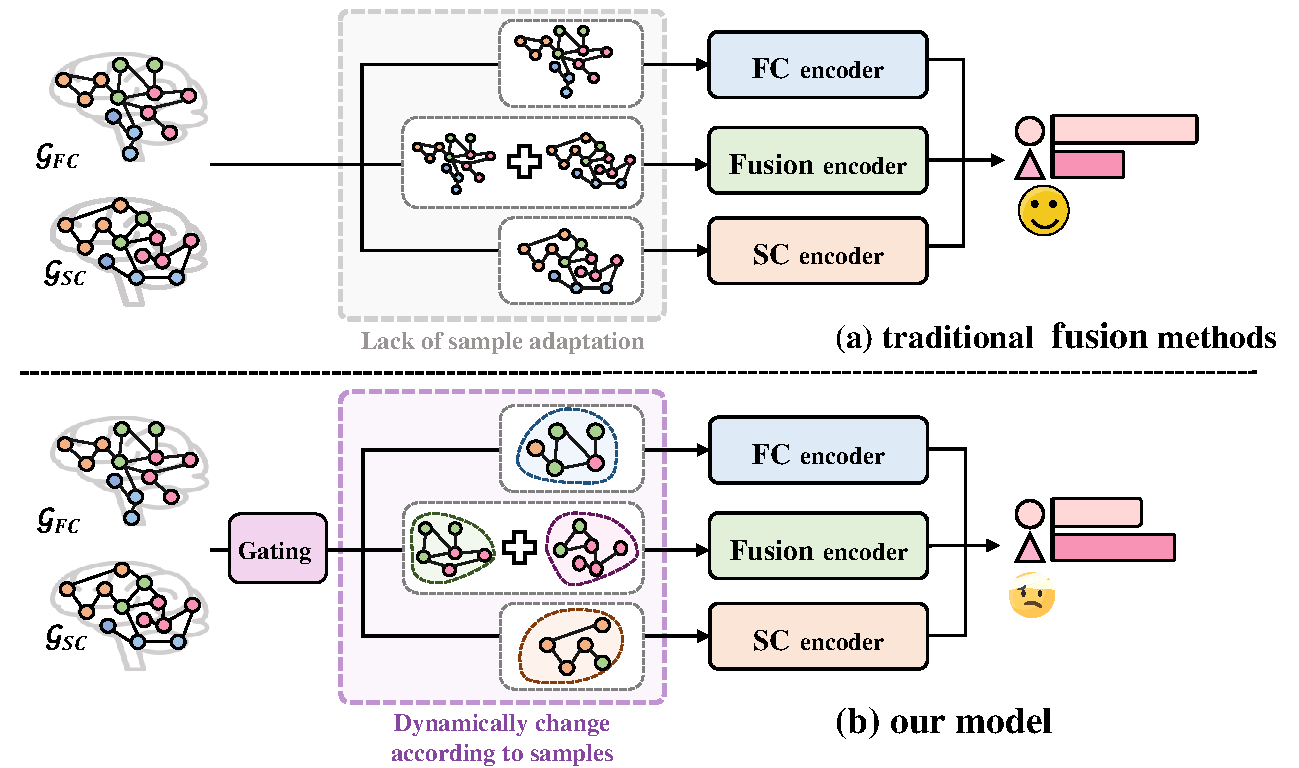
\includegraphics[width=0.96\linewidth]{toy_illustration.pdf}
    \caption{Illustration of M$^3$D-BFS. Compared with traditional methods, M$^3$D-BFS can adaptively adjust for different input samples.}
    \label{pdf_toy_illustration}
\end{figure}

% 1.    Rough territory
% 2.    Finer territory and question
% 2.5   Dynamic fusion? 
% 3.    Our contributions

\begin{figure*}[!tbp]
    \centering
    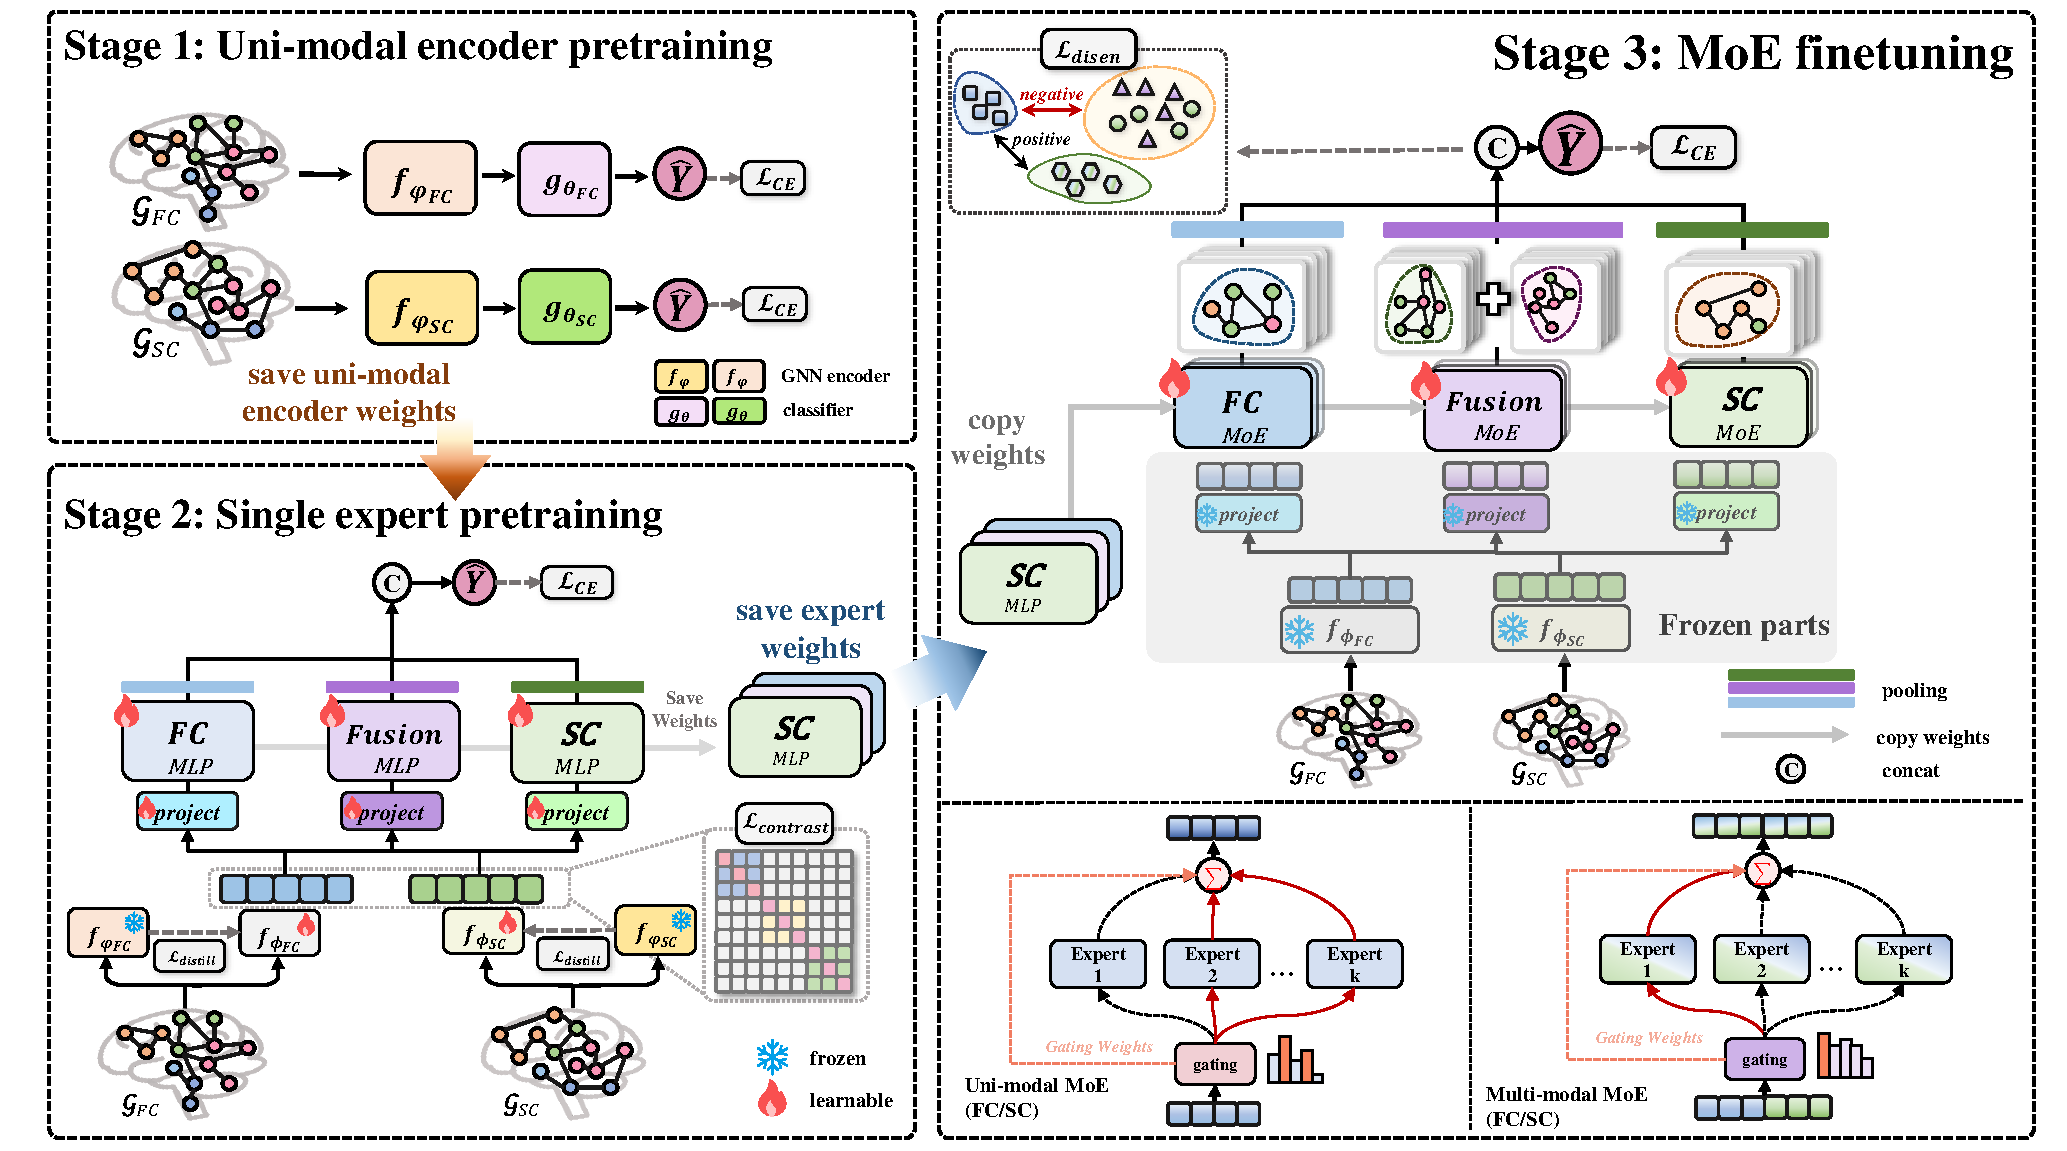
\includegraphics[width=0.92\textwidth]{M3D-BFS.pdf}
    \caption{The overall framework of our proposed M$^3$D-BFS. It consists of 3 stages: \textbf{(1) stage 1}: training for uni-modal encoders. \textbf{(2) stage 2}: pretraining of M$^3$D-BFS by using single expert. \textbf{(3) stage 3}: Finetuning M$^3$D-BFS via finetuing MoE blocks. $\mathcal{L}_{disen}$ is designed to enhance final embeddings. Structures of MoEs (uni/multi-modal) are also plotted.}
    \label{M3D-BFS}
\end{figure*}


\section{Introduction}
Most current neuroscience studies are based on uni-modal learning, involving only one modality \cite{bessadok2022graph,zahid2022brainnet,winter2024systematic}. In brain network analysis, most works focus on functional magnetic resonance imaging (fMRI) \cite{yan2019reduced} and diffusion magnetic resonance imaging (dMRI) \cite{van2020white}. However, in existing real-world medical scenarios, data from SC and FC offer complementary information \cite{chu2018function}, while single-modality-based methods are insufficient to capture comprehensive useful messages. On the other hand, multi-modal fusion, which integrates information from different modalities, can utilize data more efficiently and achieve better performance in downstream tasks, like gender classification and disorder classification.

Multi-modal brain network fusion typically utilizes data from fMRI (functional) and dMRI (structural) modalities. Different from other image-based medical fusion methods, multi-modal brain network fusion mainly considers fusion between different graphs (FC and SC) to better capture topology features from brains. In general, current fusion stategies can be divided into 3 categories: \textbf{(a) Representation-level fusion} which directly concats multi-modal representations for fusion. \cite{sebenius2021multimodal,zhang2021deep,wen2024d}. \textbf{(b) Graph-level fusion} between multi-modal brain networks. ALNEGAT \cite{chen2022adversarial} designs an attention-based adjacency matrix for fusion. Cross-GNN \cite{yang2023mapping} proproses a graph-based learning framework to capture finer inter-modal dependencies. \textbf{(c) transformer-based} fusion methods. RH-BrainFS \cite{ye2024rh} considers regional heterogeneity between SC-FC and utilized bottleneck transformer for indirect fusion. NeuroPath \cite{wei2024neuropath} adds coupling mechanism between FC and SC to improve FC's performance.

Despite the advancements in multi-modal brain network fusion, current methods are static in nature. They feed all the inputs into the same models with identical computation, ignoring the inherent difference between different input samples. In Computer Vision and Natural Language Processing, this is called multi-modal dynamic fusion, which aims to adaptively fuse multi-modal data and make predictions based on the data-wise models \cite{Cao_2023_ICCV,han2022multimodal,xue2023dynamic}. Such issue also exists in multi-modal brain network analysis, where different samples may have significant differences in strength and connectivity of some brain regions \cite{basaia2024brain,duan2017degree,chou2023functional}. While current methods treat all the samples equally by using same models to encode and fuse, they fail to avoid the effects for inherent variance among different samples during encoding and fusion. In other word, \textit{model will have better performance if it can adaptively select unimodal-wise parts and multimodal-wise parts for representation and fusion as the input sample dynamically changes.} 

To fill the gap mentioned above in neuroscience, in this work we \textbf{innovatively propose a dynamic fusion approach for sample-adaptive multi-modal brain network analysis}. As is shown in Fig. \ref{pdf_toy_illustration}, for other traditional fusion methods, all the input will be directly sent into specific or fusion modules. Our method instead adds gating module before to adaptively capture modal-specific and multi-modal data for further representation. We realize our gating module based on mixture-of-experts (MoE). However, directly adopting MoE is a challenge as it may face expert collapse in training. Therefore, we propose a \underline{\textbf{M}}ulti-stage, \underline{\textbf{M}}ulti-\underline{\textbf{M}}odal \underline{\textbf{D}}ynamic-\underline{\textbf{B}}rain \underline{\textbf{F}}u\underline{\textbf{S}}ion Strategy (\textbf{M$^3$D-BFS}). \model consists of 3 stages: We first train uni-modal encoders for SC/FC modality respectively. Then we pretrain our model by training single experts for each MoE respectively. SC-FC contrastive loss and unimodal-guided distillation loss are designed for better performance of pretraining. Finally we finetune our model by only keeping MoE modules trainable. The weights for experts in previous stage are used to initialize experts in corresponding MoEs. To further enhance final representations (uni-modal/multi-modal) and their correlations with downstream tasks, we proposed a multi-mdoal disentangle loss to better capture task-related information. To the best of our knowledge, \model is the first work for dynamic fusion in sample-wise multi-modal brain network analysis. Extensive experiments on different real-world datasets demonstrate the effectiveness of our method. 

\section{Related Works}

\noindent\textbf{Dynamic Multi-modal Fusion.} Firstly introduced in Computer Vision, dynamic fusion aims to dynamically select parts from multi-view images for fusion according to different samples \cite{han2022multimodal}. MoGE \cite{Cao_2023_ICCV} designed local gating and global gating modules for dynamic fusion. DynMM \cite{xue2023dynamic} considered dynamic scene for text-vision-audio modalities and proposed a new gating network for efficient dynamic fusion. \cite{zhang2023provable} identified the correlations between multi-modal fusion and uncertain estimation and comes up with a robust fusion method.

% \vspace{0.35em}
% \noindent\textbf{Mixture-of-Experts.} Mixture-of-Experts (MoE), composed of expert networks and a gating network, is currently used in transformer-based frameworks which replaces FFNs to accelerate computation \cite{shazeer2017outrageously,cai2024survey,lin2024moe}. In multi-modal scenes, MoE can also be used for fusion tasks. Uni-MoE \cite{li2024uni} proposed a MoE-based framwork for unified multi-modal representations. Med-MoE \cite{jiang2024med} is a lightweight framework which can tackle multiple medical tasks. MoE-LLaVA \cite{lin2024moe} incorporated MoE and learned routers to adapt MoE to LVLMs.


\vspace{0.35em}
\noindent\textbf{Multi-modal Brain Network Fusion.} To fully integrate data from different modalities for better downstream tasks, several methods have been developed for multi-modal brain network fusion. Generally, current fusion methods can be divided into three categories: \textbf{(1) Representation-level fusion} which directly concats or adds multi-modal representations before final prediction, like MMGNN \cite{sebenius2021multimodal}, GBDM \cite{zhang2021deep} and D-mhgcn \cite{wen2024d}. \textbf{(2) Graph-level fusion} which focuses on fusion graph construction. ALNEGAT \cite{chen2022adversarial} designs an Attention-based graph fusion method by learning a fusion adjancency matrix. Cross-GNN \cite{yang2023mapping} proposes a graph-based framework to capture finer cross-modal structure information. \textbf{(3) Transformer-based} fusion. RH-BrainFS  \cite{ye2024rh} uses bottleneck transformer to avoid direct interaction between SC and FC. NeuroPath \cite{wei2024neuropath} introduces coupling module between SC and FC to improve accuracy of FC-based prediction.

\section{Methodology}
\subsection{Notations}
For a given multi-modal brain network dataset, we define it as $\mathcal{D} = \{(\mathcal{G}_{SC}^i, \mathcal{G}_{FC}^i), y_i\}_{i=1}^{n}$, where $n$ represents the sample size. For each sample, $\mathcal{G}_{SC}^i, \mathcal{G}_{FC}^i$ stands for structural connectivity graph and functional connectivity graph respectively, and $y_i$ is the corresponding label (depending on different tasks, gender, disease, etc) and $y_i \in \{0,1\}$. For brain network of each modality: $\mathcal{G}_{m} = (A_m, X_m, \mathcal{V}_{m}, \mathcal{E}_{m}), m \in \{SC, FC\}$, nodes $\mathcal{V}_m$ represents different brain regions in the brain while edges $\mathcal{E}_m$ represents the connectivity between two brain regions. $X_m\in\mathbb{R}^{N\times d}$ denotes node features for each region and $A_m \in \mathbb{R}^{N \times N}$ denotes the adjacency matrix for brain network $\mathcal{G}_m$.

\subsection{Overview of M$^3$D-BFS}
In this section, we will introduce more details about our M$^3$D-BFS. The structure of our framework is shown in Fig. \ref{M3D-BFS} (stage 3), we project uni-modal embeddings and send them into following MoE blocks. Via MoE's gating mechanism, different brain regions can be assigned to following experts dynamically, thus realizing sample-adaptive dynamic fusion. To facilitate better training, we divide our M$^3$D-BFS into 3 stages: \textbf{(1) stage 1: Uni-modal encoder pretraining}, where we train SC and FC encoders respectively. \textbf{(2) stage 2: Single expert pretraining}, where we train our multi-modal fusion model using single expert network for SC/FC/Fusion. \textbf{(3) stage 3: MoE finetuning} for dynamic multi-modal fusion, where we finetune MoE blocks while keeping other modules frozen. 
% Model weights for single experts from stage 2 are utilized as initialization weights for corresponding MoEs. 
% The framework of our model is shown in Fig. \ref{M3D-BFS}.

\subsection{Uni-modal encoder pretraining}
Directly training a multi-modal fusion model can lead to sub-optimal performance, sometimes the performance of the fusion model can be worse than uni-modal models. This phenomenon of insufficient learning during multi-modal fusion is called ``modality laziness'' \cite{du2023uni} which hurts fusion model's generalization ability. 

Thus, encouraged by \cite{du2023uni}, we first train uni-modal encoders for FC/SC respectively, which \textbf{serve as guidance for multi-modal encoder in stage 2}. Formally, for given data $\{(\mathcal{G}_{FC}^i, \mathcal{G}_{SC}^i), y_i\}$ which stands for $i\mbox{-}th$ sample, we denote the uni-modal encoder as:
\begin{small}
\begin{equation}
    \hat{y_i}_m = g_{\theta_m}\circ f_{\varphi_m}(\mathcal{G}_{m}^i) = g_{\theta_m}(f_{\varphi_m}(\mathcal{G}_{m}^i))
    \label{uni-enc}
\end{equation}
\end{small}
Here $m \in \{SC,FC\}$. $f_{\varphi_m}$ denotes the encoder and here we realize it with a two-layer GCN. $g_{\theta_m}$ is for classifier and we use a one-layer MLP (multi-layer perceptron) for implementation. For either SC or FC, we use cross-entropy loss ($\mathcal{L}_{ce}$) to optimize the uni-modal model. 
% \begin{small}
% \begin{equation}
%     \mathcal{L}_{stage1} = \mathcal{L}_{ce} = - \sum_{i=0}^{N} y_i \cdot \log \hat{y_i} + (1-y_i)\cdot \log (1-\hat{y_i})
% \end{equation}
% \end{small}

After uni-modal training, we save the weights for SC/FC encoders ($f_{\varphi_{SC}}, f_{\varphi_{FC}}$), which will be used for soft alignment in stage 2.


\subsection{Single expert pretraining}
We train our multi-modal fusion model after we pretrain uni-modal encoders. However, directly training MoE is challenging in practice, which may lead to instability during training process \cite{shazeer2017outrageously}. 

According to \cite{li2024uni,lin2024moe,chen2024eve}, progressive training strategy is an effective way to train powerful MoE models. To this end, we further adopt a \textbf{``pretrain then finetune'' paradigm} for MoE training \cite{li2024uni}. Formally, we first train single expert then finetune the MoEs. M$^3$D-BFS is independent of the specific architecture of MoE experts and here we utilize MLP as our expert network. For representations from SC/FC encoders (denote as $h_{SC}, h_{FC}$), we project and feed them into following experts.  Corresponding to our design of MoEs, we consider three types of expert MLPs: FC-specific, SC-specific and Fusion experts. Modal-specific experts take the representation of uni-modal as input while Fusion expert takes the concatenation of SC and FC. $\textbf{READOUT}(\cdot)$ will be applied for the output of each expert before concatenation and final prediction (shown in Eq. \ref{equ_stage2}, and $\textbf{FFN}(\cdot)$ is the feedforward network layer).
\begin{small}
\begin{equation}
\begin{aligned}
\begin{cases}
    \label{equ_stage2}
    \hat{y_i} &= \textbf{FFN}(\text{Concat}(z_{SC}^i , \ z_{FC}^i , \ z_{Fusion}^i))
    \\
    z^i_m &= \textbf{READOUT}(h_m^i), m \in \{SC, FC, Fusion\}
\end{cases}
\end{aligned}
\end{equation}
\end{small}

However, simple cross-entropy loss ($\mathcal{L}_{ce}$) is not enough for multi-modal supervised learning and the reasons lie in label's insufficient supervision for different modalities. Therefore, we add the supervision of pretrained uni-modal encoders from stage 1 \cite{du2023uni}. For representations through encoders $(f_{\phi_{SC}}, f_{\phi_{FC}})$ from stage 1, we design a uni-modal guided distillation loss as follows:
\begin{small}
    \begin{equation}
        \mathcal{L}_{distill} = \frac{\tau^2}{2} \bigg ( \mathcal D_{KL}(\frac{h_{\varphi_{FC}}}{\tau},\frac{h_{\phi_{FC}}}{\tau}) + \mathcal{D}_{KL}(\frac{h_{\varphi_{SC}}}{\tau},\frac{h_{\phi_{SC}}}{\tau})\bigg )
    \end{equation}
\end{small}

The output of the uni-modal encoders from stage 2 are denoted as ($h_{\phi_{SC}}, h_{\phi_{FC}}$) and we regard stage 1 representations as teacher logits $(h_{\varphi_{SC}}, h_{\varphi_{FC}})$. Through $\mathcal{L}_{distill}$ as soft alignment, our \model can keep the performance of uni-modal encoders.

Besides, for better SC/FC representations, we adopt practice from LIMoE \cite{mustafa2022multimodal} pretraining which utilized CLIP-based loss \cite{radford2021learning} between batch data. For given SC/FC representations $(h_{\phi_{SC}}, h_{\phi_{FC}}) \in \mathbb{R}^{N \times d}$, we utilize \underline{\textbf{C}}ontrastive \underline{\textbf{M}}ultimodal \underline{\textbf{B}}rain \underline{\textbf{P}}re-training loss (\textbf{CMBP}, denote as $\mathcal{L}_{contrast}$) for better align representations between SC and FC. We use pooling for $(h_{\phi_{SC}}, h_{\phi_{FC}})$, and get $d$-dimension representations for SC and FC modality.
% $(\overline{h}_{\phi_{SC}}, \overline{h}_{\phi_{FC}}) \in \mathbb{R}^d$.
$\mathcal{L}_{contrast}$ minimizes the distance between paired SC-FC data within one batch during training: 
 $\mathcal{L}_{contrast} = \frac{1}{2}(\mathcal{L}_{S2F} + \mathcal{L}_{F2S})$. Here we use $\textbf{InfoNCE}(\cdot)$ for implementation.

During this stage, classification loss $\mathcal{L}_{ce}$, distillation loss $\mathcal{L}_{distill}$ and $\mathcal{L}_{contrast}$ together make the loss function (Eq. \ref{equ_loss_s2}, where $\beta$ is a hyper-parameter ranging $(0,1)$).
\begin{equation}
    \mathcal{L}_{stage2} = \mathcal{L}_{ce} + \beta\cdot(\mathcal{L}_{distill} + \mathcal{L}_{contrast})
    \label{equ_loss_s2}
\end{equation}

After training, we save the weights of single MLP experts (SC, FC, Fusion), which will be used in stage 3.


\begin{table*}[!htbp]
    \centering
    % \small
% \setlength{\tabcolsep}{1mm}
    \caption{Comparison results on two different datasets (HCP, ZDXX). We run 10 times and record average acc $\pm$ std (\%). The best results are marked \textbf{bold}, the second best \underline{underline} and the third best \colorbox{lightgray}{gray}.}
    \resizebox{0.9\textwidth}{!}{
    \begin{tabular}{clcccccc}
        \toprule
        \multirow{1}{*}{\textbf{Datasets}} &
        \multirow{1}{*}{\textbf{Methods}} &
        \multirow{1}{*}{\textbf{Modality}} &
        \textbf{ACC} & \textbf{SEN} & \textbf{SPE} & \textbf{F1} & \textbf{AUC}
        % \textbf{Avg.Rank}
        \\
        \midrule
        \multirow{12}{*}{\Large{\textbf{HCP}}}
        & GCN & FC & 64.03 $\pm$ \scriptsize{1.21} & 55.01 $\pm$ \scriptsize{2.88} & 71.75 $\pm$ \scriptsize{2.37} & 57.15 $\pm$ \scriptsize{2.49} & 63.38 $\pm$ \scriptsize{1.25}
        \\
        & GCN & SC & 68.23 $\pm$ \scriptsize{1.76} & 66.22 $\pm$ \scriptsize{4.79} & 72.27 $\pm$ \scriptsize{4.53} & 67.91 $\pm$ \scriptsize{2.71} & 69.61 $\pm$ \scriptsize{1.75}
        \\
        & BrainNPT & FC & 67.78 $\pm$ \scriptsize{1.53} & 60.67 $\pm$ \scriptsize{1.34} & 73.98 $\pm$ \scriptsize{2.83} & 59.15 $\pm$ \scriptsize{3.70} & 66.97 $\pm$ \scriptsize{2.44}
        \\
        & BrainNPT & SC & 70.74 $\pm$ \scriptsize{1.49} & 68.95 $\pm$ \scriptsize{4.82} & 70.02 $\pm$ \scriptsize{5.67} & 68.16 $\pm$ \scriptsize{2.13} & 70.11 $\pm$ \scriptsize{1.73}
        \\
        \cmidrule{2-8}
        % \multirow{8}{*}{\textbf{HCP}}
        & SVM & FC, SC &  74.49 $\pm$ \scriptsize{2.97} & 71.18 $\pm$ \scriptsize{4.95} & 77.32 $\pm$ \scriptsize{3.30} & 71.96 $\pm$ \scriptsize{3.49} & 74.25 $\pm$ \scriptsize{3.05} 
        \\
        & Random Forest & FC, SC & 68.24 $\pm$ \scriptsize{2.94} & 54.88 $\pm$ \scriptsize{5.78} & 79.64 $\pm$ \scriptsize{4.16} & 61.31 $\pm$ \scriptsize{4.44} & 67.26 $\pm$ \scriptsize{3.04}
        \\
        & MMGNN & FC, SC & 73.33 $\pm$ \scriptsize{2.82} & 71.17 $\pm$ \scriptsize{4.52} & 75.17 $\pm$ \scriptsize{5.67} & 71.10 $\pm$ \scriptsize{2.88} & 73.17 $\pm$ \scriptsize{2.72}
        \\
        & AL-NEGAT & FC, SC & 75.12 $\pm$ \scriptsize{3.66} & 72.86 $\pm$ \scriptsize{7.74} & \underline{84.46 $\pm$ \scriptsize{5.05}} & 76.13 $\pm$ \scriptsize{4.70} & \colorbox{lightgray}{78.66 $\pm$ \scriptsize{3.81} }
        \\
        & Cross-GNN & FC, SC & \underline{78.93 $\pm$ \scriptsize{1.05}} & 73.53 $\pm$ \scriptsize{1.84} & \textbf{85.04 $\pm$ \scriptsize{2.02}} & \textbf{76.81 $\pm$ \scriptsize{0.86}} & \underline{79.82 $\pm$ \scriptsize{0.72}}
        \\
        & RH-BrainFS & FC, SC & \colorbox{lightgray}{78.63 $\pm$ \scriptsize{4.36}} & \underline{75.59 $\pm$ \scriptsize{6.75}} & 81.25 $\pm$ \scriptsize{6.04} & \colorbox{lightgray}{76.49 $\pm$ \scriptsize{6.91}} & 78.42 $\pm$ \scriptsize{4.38}
        \\
        & NeuroPath & FC, SC & 77.77 $\pm$ \scriptsize{1.87}  & \colorbox{lightgray}{75.24 $\pm$ \scriptsize{2.61}}  & 80.38 $\pm$ \scriptsize{1.50} & 75.78 $\pm$ \scriptsize{1.84} & 77.81 $\pm$ \scriptsize{1.67}
        \\
        \cmidrule{2-8}
        & \textbf{\model (Ours)} & FC, SC & \textbf{81.21 $\pm$ \scriptsize{0.85}} & \textbf{76.14 $\pm$ \scriptsize{3.32}}  & \colorbox{lightgray}{82.50 $\pm$ \scriptsize{3.07}}  & \underline{76.75 $\pm$ \scriptsize{1.25}} & \textbf{80.80 $\pm$ \scriptsize{1.07}}
        \\

        %--------------------- dataset zhongdaxinxiang --------------------------%
        \midrule\midrule
        \multirow{12}{*}{\Large{\textbf{zhongdaxinxiang}}}
        & GCN & FC & 68.63 $\pm$ \scriptsize{1.28} & 64.61 $\pm$ \scriptsize{4.67} & 72.68 $\pm$ \scriptsize{4.52} & 64.68 $\pm$ \scriptsize{3.13} & 68.64 $\pm$ \scriptsize{1.18}
        \\
        & GCN & SC & 72.15 $\pm$ \scriptsize{2.49} & 72.79 $\pm$ \scriptsize{5.14} & 73.24 $\pm$ \scriptsize{4.80} & 71.90 $\pm$ \scriptsize{4.25} & 72.02 $\pm$ \scriptsize{2.52}
        \\
        & BrainNPT & FC & 70.65 $\pm$ \scriptsize{1.85} & 73.00 $\pm$ \scriptsize{4.59} & 69.01 $\pm$ \scriptsize{4.30} & 69.27 $\pm$ \scriptsize{2.64} & 71.00 $\pm$ \scriptsize{2.03}
        \\
        & BrainNPT & SC & 72.83 $\pm$ \scriptsize{1.73} & 74.57 $\pm$ \scriptsize{3.80} & 69.89 $\pm$ \scriptsize{3.87} & 73.63 $\pm$ \scriptsize{4.07} & 72.78 $\pm$ \scriptsize{2.65}
        \\
        \cmidrule{2-8}
        % \multirow{8}{*}{\textbf{zhongdaxinxiang}}
        & SVM & FC, SC &  66.06 $\pm$ \scriptsize{1.56} & 58.01 $\pm$ \scriptsize{2.49} & 74.04 $\pm$ \scriptsize{1.77} & 62.03 $\pm$ \scriptsize{2.27} & 66.03 $\pm$ \scriptsize{1.56} 
        \\
        & Random Forest & FC, SC & 62.43 $\pm$ \scriptsize{2.19} & 56.17 $\pm$ \scriptsize{2.87} & 68.60 $\pm$ \scriptsize{3.48} & 59.04 $\pm$ \scriptsize{2.73} & 62.38 $\pm$ \scriptsize{2.20}
        \\
        & MMGNN & FC, SC & 59.72 $\pm$ \scriptsize{3.18} & 65.10 $\pm$ \scriptsize{4.83} & 54.42 $\pm$ \scriptsize{4.42} & 59.96 $\pm$ \scriptsize{4.02} & 59.76 $\pm$ \scriptsize{3.15}
        \\
        & AL-NEGAT & FC, SC & 71.86 $\pm$ \scriptsize{2.49} & 75.26 $\pm$ \scriptsize{3.62} & 68.12 $\pm$ \scriptsize{6.19} & 72.16 $\pm$ \scriptsize{2.24} & 71.69 $\pm$ \scriptsize{2.56}
        \\
        & Cross-GNN & FC, SC & 74.01 $\pm$ \scriptsize{2.33} & \textbf{77.39 $\pm$ \scriptsize{5.71}} & 70.46 $\pm$ \scriptsize{5.65} & 74.38 $\pm$ \scriptsize{3.15} & 73.92 $\pm$ \scriptsize{2.33}
        \\
        & RH-BrainFS & FC, SC & \underline{78.48 $\pm$ \scriptsize{1.43}} & 76.20 $\pm$ \scriptsize{4.06} & \underline{80.72 $\pm$ \scriptsize{3.60}} & \colorbox{lightgray}{77.35 $\pm$ \scriptsize{1.97}} & \colorbox{lightgray}{78.46 $\pm$ \scriptsize{1.43}}
        \\
        & NeuroPath & FC, SC & \colorbox{lightgray}{78.01 $\pm$ \scriptsize{1.17}} & \colorbox{lightgray}{77.03 $\pm$ \scriptsize{2.23}} & \colorbox{lightgray}{79.17 $\pm$ \scriptsize{3.47}} & \underline{77.54 $\pm$ \scriptsize{2.28}} & \underline{78.50 $\pm$ \scriptsize{1.24}}
        \\
        \cmidrule{2-8}
        & \textbf{\model (Ours)} & FC, SC & \textbf{80.85 $\pm$ \scriptsize{2.44}} & \underline{77.22 $\pm$ \scriptsize{3.04}} & \textbf{83.91 $\pm$ \scriptsize{4.95}} & \textbf{77.82 $\pm$ \scriptsize{3.62}} & \textbf{80.74 $\pm$ \scriptsize{2.57}}
        \\
        
        
        \bottomrule
    \end{tabular}    
    } 
    \label{table_comp_HCP}
\end{table*}    



%-----------------------stage 3------------------------------------%
% \subsection{Stage 3: MoE-based finetuning for dynamic multi-modal fusion}
\subsection{MoE finetuning}
\noindent\textbf{MoE finetuning for dynamic multi-modal fusion. }Based on the pretrained model in stage 2, We finally finetune our \model in stage 3 to make our training process more stable. In this stage we replace the MLP experts with MoEs, whose experts have the same structure as MLP experts. As is shown in Fig. \ref{M3D-BFS}, We only train MoEs during this stage while keeping other modules frozen. We consider three types of MoEs: Uni-modal MoEs (SC-specific, FC-specific) which capture SC-only or FC-only features and Multi-modal MoE which dynamically fuses SC and FC features. Moreover, to avoid insufficient learning for some experts in MoE training, we apply the MLP weights saved in stage 2 to initialize all the expert networks in corresponding MoEs. 

Each MoE consists of two parts: expert networks and gating network. Here we follow the classical practice from \cite{shazeer2017outrageously} and use MLP to realize both modules. For MoE $m$ which denotes its type ($m \in \{\ SC, FC, Fusion\}$), the output can be written as follows:
\begin{small}
\begin{equation}
    y_m = \sum_{i=1}^{N_m} G_m(h_m)_i \cdot E_m(h_m)_i
\end{equation}
\end{small}

Where the input $h_m$ takes the dimension of $\mathbb{R}^{N\times d}$ for $m \in \{SC, FC\}$ ($N_m=N$) and $\mathbb{R}^{2N\times d}$ for $m\in \{Fusion\}$ ($N_m=2N$). $G_m$ is gating network for corresponding MoE. Following \cite{shazeer2017outrageously}, we apply \textbf{Softmax} function for gating output. Before taking softmax, we add Gaussian noise and only keep top k values. Here we set k as 1, which means each brain region selects only one expert during training and inference. As the output of $G_m$ depends on input $X$, it can dynamically assign brain regions to different experts according to different data samples.

However, direct training process can get collapsed easily, where all input can be assigned to only one expert, and distributions of gating network can be imbalanced, where favored experts are trained more rapidly and are preferred during inference while other experts will get insufficient training \cite{chi2022representation,shazeer2017outrageously}. Thus MoE will degenerate into a single expert. To alleviate this issue of imbalanced training between experts, we apply the Importance loss and Load loss for each MoE ($\mathcal{L}_{moe}$). For given MoE, the loss is the combination of $\mathcal{L}_{Importance}$ and $\mathcal{L}_{load}$,
% \begin{small}
% \begin{equation}
% \mathcal{L}_{moe} = \mathcal{L}_{Importance} + \mathcal{L}_{Load}
% \label{equ_moe_total}
% \end{equation}
% \end{small}
where the importance loss and load loss are defined as:
\begin{small}
\begin{equation}
\begin{cases}
\begin{aligned}
    \mathcal{L}_{Importance}(X) &= CV(Importance(X))^2 = CV(\sum_{x\in X}G(x))^2
    \\
    \mathcal{L}_{Load}(X) &= CV(Load(X))^2 = CV(\sum_{x\in X}P(x))^2
    \label{equ_moe}
\end{aligned}
\end{cases}
\end{equation}
\end{small}
Here $CV(\cdot)$ means the coefficient of variation of the values. The initialization of experts' weights, as well as the MoE loss function together alleviate imbalanced training issue of MoE which makes the training more stable and more efficient.

% \begin{figure}
%     \centering
%     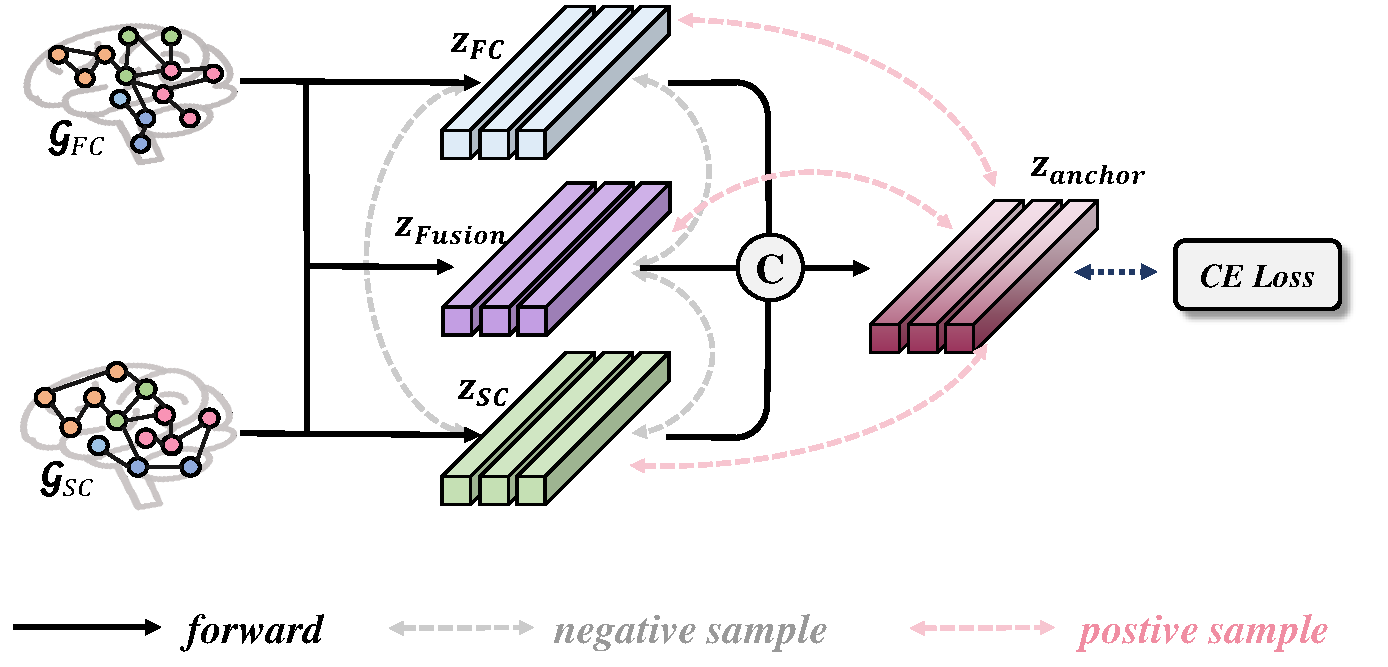
\includegraphics[width=0.96\linewidth]{disen.pdf}
%     \caption{The process of multi-modal disentanglement loss. Representations from different modalities are regarded as negative samples while $z_{anchor}$ for prediction functions as positive sample.}
%     \label{pdf_disen}
% \end{figure}

% \subsection{Representation-enhanced multi-modal disentanglement loss}
\vspace{0.35em}
\noindent\textbf{Representation-enhanced multi-modal disentanglement loss.} In multi-modal learning, insufficient label information for supervision may influence the performance for modal-specific and fusion embeddings. One solution is through disentangled representation learning which reduces redundancy between modal-specific and modal-fusion information while keeping their correlations with label. Here, derived from \cite{li2022modeling}'s method, we design our multi-mdoal disentanglement loss to learn better uni-modal and multi-modal representations ($\mathcal{L}_{disen}$). We apply pooling function after the output of MoE and for each data, the final embeddings are $\{z_{SC}, z_{FC}, z_{Fusion}\} \in \mathbb{R}^d$. Our $\mathcal{L}_{disen}$ is based on contrastive loss and we hope that the final embeddings can be as orthogonal to each other as possible for better representation. We use the concatenation of three representations and get the anchor sample for $i\mbox{-}th$ data $z^i_{anchor}$ by concating $ z^i_{SC}, z^i_{FC}$ and $z^i_{Fusion}$. 
% \begin{small}
% \begin{equation}
%     z_{anchor}^i = \textbf{FFN}(z^i_{SC} \ || \ z^i_{FC} \ || \ z^i_{Fusion})
% \end{equation}
% \end{small}
$z^i_{anchor} \in \mathbb{R}^d$ is used for prediction and for each $z_m^i$, we regard other types as negative samples and $z^i_{anchor}$ as positive sample. 
% The process is shown in Fig. \ref{pdf_disen} and 
$\mathcal{L}_{disen}$ can be written as Eq. \ref{equ_loss_disen}:
\begin{small}
\begin{equation}
\begin{aligned}
&\mathcal{L}_{disen} =  -\frac{1}{n\cdot M}\sum_{i=1}^{n}\sum_{m=1}^{M}
\\
&  \quad 
% \Big( 
\log
\frac{
\exp 
    \big(
        \frac{z_m^i \cdot z_{anchor}^{i}}{\tau_d} 
    \big)
}
{
\exp\big(
        \frac{z_m^i \cdot z_{anchor}^{i}}{\tau_d} 
    \big) + 
    \sum_{\substack{q=1, \\ q \not = m}}^{M} \exp \big(
                                    \frac{z_m^i \cdot z_q^i}{\tau_d}
                                    \big)
}
% \Big)
\label{equ_loss_disen}
\end{aligned}
\end{equation}
\end{small}

Here $M$ defers to different types ($\{SC, FC, Fusion\}$). According to Eq. \ref{equ_loss_disen}, through $\mathcal{L}_{disen}$, we can disentangle different representations while increasing their relevance to downstream tasks, thus enhancing their representations.
Finally, the loss function in stage 3 is in Eq. \ref{equ_loss_stage3} with $\alpha \in (0,1)$:

\begin{small}
\begin{equation}
    \mathcal{L}_{stage3} = \mathcal{L}_{ce} + \alpha \cdot \mathcal{L}_{moe} + (1-\alpha)\cdot \mathcal{L}_{disen}
    \label{equ_loss_stage3}
\end{equation}
\end{small}



%------------------------------------- Experiments --------------------------------------%



% \begin{table*}[!htbp]
    \centering
    % \small
% \setlength{\tabcolsep}{1mm}
    \caption{Comparison results on two different datasets (HCP, ZDXX). We run 10 times and record average acc $\pm$ std (\%). The best results are marked \textbf{bold}, the second best \underline{underline} and the third best \colorbox{lightgray}{gray}.}
    \resizebox{0.9\textwidth}{!}{
    \begin{tabular}{clcccccc}
        \toprule
        \multirow{1}{*}{\textbf{Datasets}} &
        \multirow{1}{*}{\textbf{Methods}} &
        \multirow{1}{*}{\textbf{Modality}} &
        \textbf{ACC} & \textbf{SEN} & \textbf{SPE} & \textbf{F1} & \textbf{AUC}
        % \textbf{Avg.Rank}
        \\
        \midrule
        \multirow{12}{*}{\Large{\textbf{HCP}}}
        & GCN & FC & 64.03 $\pm$ \scriptsize{1.21} & 55.01 $\pm$ \scriptsize{2.88} & 71.75 $\pm$ \scriptsize{2.37} & 57.15 $\pm$ \scriptsize{2.49} & 63.38 $\pm$ \scriptsize{1.25}
        \\
        & GCN & SC & 68.23 $\pm$ \scriptsize{1.76} & 66.22 $\pm$ \scriptsize{4.79} & 72.27 $\pm$ \scriptsize{4.53} & 67.91 $\pm$ \scriptsize{2.71} & 69.61 $\pm$ \scriptsize{1.75}
        \\
        & BrainNPT & FC & 67.78 $\pm$ \scriptsize{1.53} & 60.67 $\pm$ \scriptsize{1.34} & 73.98 $\pm$ \scriptsize{2.83} & 59.15 $\pm$ \scriptsize{3.70} & 66.97 $\pm$ \scriptsize{2.44}
        \\
        & BrainNPT & SC & 70.74 $\pm$ \scriptsize{1.49} & 68.95 $\pm$ \scriptsize{4.82} & 70.02 $\pm$ \scriptsize{5.67} & 68.16 $\pm$ \scriptsize{2.13} & 70.11 $\pm$ \scriptsize{1.73}
        \\
        \cmidrule{2-8}
        % \multirow{8}{*}{\textbf{HCP}}
        & SVM & FC, SC &  74.49 $\pm$ \scriptsize{2.97} & 71.18 $\pm$ \scriptsize{4.95} & 77.32 $\pm$ \scriptsize{3.30} & 71.96 $\pm$ \scriptsize{3.49} & 74.25 $\pm$ \scriptsize{3.05} 
        \\
        & Random Forest & FC, SC & 68.24 $\pm$ \scriptsize{2.94} & 54.88 $\pm$ \scriptsize{5.78} & 79.64 $\pm$ \scriptsize{4.16} & 61.31 $\pm$ \scriptsize{4.44} & 67.26 $\pm$ \scriptsize{3.04}
        \\
        & MMGNN & FC, SC & 73.33 $\pm$ \scriptsize{2.82} & 71.17 $\pm$ \scriptsize{4.52} & 75.17 $\pm$ \scriptsize{5.67} & 71.10 $\pm$ \scriptsize{2.88} & 73.17 $\pm$ \scriptsize{2.72}
        \\
        & AL-NEGAT & FC, SC & 75.12 $\pm$ \scriptsize{3.66} & 72.86 $\pm$ \scriptsize{7.74} & \underline{84.46 $\pm$ \scriptsize{5.05}} & 76.13 $\pm$ \scriptsize{4.70} & \colorbox{lightgray}{78.66 $\pm$ \scriptsize{3.81} }
        \\
        & Cross-GNN & FC, SC & \underline{78.93 $\pm$ \scriptsize{1.05}} & 73.53 $\pm$ \scriptsize{1.84} & \textbf{85.04 $\pm$ \scriptsize{2.02}} & \textbf{76.81 $\pm$ \scriptsize{0.86}} & \underline{79.82 $\pm$ \scriptsize{0.72}}
        \\
        & RH-BrainFS & FC, SC & \colorbox{lightgray}{78.63 $\pm$ \scriptsize{4.36}} & \underline{75.59 $\pm$ \scriptsize{6.75}} & 81.25 $\pm$ \scriptsize{6.04} & \colorbox{lightgray}{76.49 $\pm$ \scriptsize{6.91}} & 78.42 $\pm$ \scriptsize{4.38}
        \\
        & NeuroPath & FC, SC & 77.77 $\pm$ \scriptsize{1.87}  & \colorbox{lightgray}{75.24 $\pm$ \scriptsize{2.61}}  & 80.38 $\pm$ \scriptsize{1.50} & 75.78 $\pm$ \scriptsize{1.84} & 77.81 $\pm$ \scriptsize{1.67}
        \\
        \cmidrule{2-8}
        & \textbf{\model (Ours)} & FC, SC & \textbf{81.21 $\pm$ \scriptsize{0.85}} & \textbf{76.14 $\pm$ \scriptsize{3.32}}  & \colorbox{lightgray}{82.50 $\pm$ \scriptsize{3.07}}  & \underline{76.75 $\pm$ \scriptsize{1.25}} & \textbf{80.80 $\pm$ \scriptsize{1.07}}
        \\

        %--------------------- dataset zhongdaxinxiang --------------------------%
        \midrule\midrule
        \multirow{12}{*}{\Large{\textbf{zhongdaxinxiang}}}
        & GCN & FC & 68.63 $\pm$ \scriptsize{1.28} & 64.61 $\pm$ \scriptsize{4.67} & 72.68 $\pm$ \scriptsize{4.52} & 64.68 $\pm$ \scriptsize{3.13} & 68.64 $\pm$ \scriptsize{1.18}
        \\
        & GCN & SC & 72.15 $\pm$ \scriptsize{2.49} & 72.79 $\pm$ \scriptsize{5.14} & 73.24 $\pm$ \scriptsize{4.80} & 71.90 $\pm$ \scriptsize{4.25} & 72.02 $\pm$ \scriptsize{2.52}
        \\
        & BrainNPT & FC & 70.65 $\pm$ \scriptsize{1.85} & 73.00 $\pm$ \scriptsize{4.59} & 69.01 $\pm$ \scriptsize{4.30} & 69.27 $\pm$ \scriptsize{2.64} & 71.00 $\pm$ \scriptsize{2.03}
        \\
        & BrainNPT & SC & 72.83 $\pm$ \scriptsize{1.73} & 74.57 $\pm$ \scriptsize{3.80} & 69.89 $\pm$ \scriptsize{3.87} & 73.63 $\pm$ \scriptsize{4.07} & 72.78 $\pm$ \scriptsize{2.65}
        \\
        \cmidrule{2-8}
        % \multirow{8}{*}{\textbf{zhongdaxinxiang}}
        & SVM & FC, SC &  66.06 $\pm$ \scriptsize{1.56} & 58.01 $\pm$ \scriptsize{2.49} & 74.04 $\pm$ \scriptsize{1.77} & 62.03 $\pm$ \scriptsize{2.27} & 66.03 $\pm$ \scriptsize{1.56} 
        \\
        & Random Forest & FC, SC & 62.43 $\pm$ \scriptsize{2.19} & 56.17 $\pm$ \scriptsize{2.87} & 68.60 $\pm$ \scriptsize{3.48} & 59.04 $\pm$ \scriptsize{2.73} & 62.38 $\pm$ \scriptsize{2.20}
        \\
        & MMGNN & FC, SC & 59.72 $\pm$ \scriptsize{3.18} & 65.10 $\pm$ \scriptsize{4.83} & 54.42 $\pm$ \scriptsize{4.42} & 59.96 $\pm$ \scriptsize{4.02} & 59.76 $\pm$ \scriptsize{3.15}
        \\
        & AL-NEGAT & FC, SC & 71.86 $\pm$ \scriptsize{2.49} & 75.26 $\pm$ \scriptsize{3.62} & 68.12 $\pm$ \scriptsize{6.19} & 72.16 $\pm$ \scriptsize{2.24} & 71.69 $\pm$ \scriptsize{2.56}
        \\
        & Cross-GNN & FC, SC & 74.01 $\pm$ \scriptsize{2.33} & \textbf{77.39 $\pm$ \scriptsize{5.71}} & 70.46 $\pm$ \scriptsize{5.65} & 74.38 $\pm$ \scriptsize{3.15} & 73.92 $\pm$ \scriptsize{2.33}
        \\
        & RH-BrainFS & FC, SC & \underline{78.48 $\pm$ \scriptsize{1.43}} & 76.20 $\pm$ \scriptsize{4.06} & \underline{80.72 $\pm$ \scriptsize{3.60}} & \colorbox{lightgray}{77.35 $\pm$ \scriptsize{1.97}} & \colorbox{lightgray}{78.46 $\pm$ \scriptsize{1.43}}
        \\
        & NeuroPath & FC, SC & \colorbox{lightgray}{78.01 $\pm$ \scriptsize{1.17}} & \colorbox{lightgray}{77.03 $\pm$ \scriptsize{2.23}} & \colorbox{lightgray}{79.17 $\pm$ \scriptsize{3.47}} & \underline{77.54 $\pm$ \scriptsize{2.28}} & \underline{78.50 $\pm$ \scriptsize{1.24}}
        \\
        \cmidrule{2-8}
        & \textbf{\model (Ours)} & FC, SC & \textbf{80.85 $\pm$ \scriptsize{2.44}} & \underline{77.22 $\pm$ \scriptsize{3.04}} & \textbf{83.91 $\pm$ \scriptsize{4.95}} & \textbf{77.82 $\pm$ \scriptsize{3.62}} & \textbf{80.74 $\pm$ \scriptsize{2.57}}
        \\
        
        
        \bottomrule
    \end{tabular}    
    } 
    \label{table_comp_HCP}
\end{table*}    


\section{Experiments}
% To further illustrate the effectiveness of our M$^3$D-BFS, we conduct extensive experiments on different multi-modal brain datasets. Generally, we conduct our experiments aiming to answer following questions, each of which will be discussed in the corresponding subsections:

% \vspace{0.35em}
% \noindent \textbf{Q1:} Does \model improve the performance compared to uni-modal models? \\
% \noindent \textbf{Q2:} What's the performance of \model compared with state-of-the-art (SOTA) fusion methods? \\
% \noindent \textbf{Q3:} Do different sub-modules of \model works? \\
% \noindent \textbf{Q4:} How do different hyper-parameters influence model's performance? \\
% \noindent \textbf{Q5:} Are experts in MoEs fully utilized during inference?

\subsection{Experimental settings}
\textbf{Datasets.} We evaluate our \model on two different datasets: \textbf{(1) Human Connectsome Project (HCP)} \cite{HCP}, a public dataset on gender classification which consists of 560 female and 479 male samples. \textbf{(2) Major Depressive Disorder dataset from hospitals (zhongdaxinxiang, also short as ZDXX)}, including the Affiliated Zhongda Hospital of Southeast University and  the Second Affiliated Hospital of Xinxiang Medical University, which consists of 94 controls and 93 MDD patients.

We also introduce preprocess of our dataset. \textbf{(1) SC}: The brain's diffusion toolbox of FMRIB is utilized dMRI preprocessing \cite{FMRIB}. Then the brain regions are obtained ($\mathcal{V}_{SC}$) through Anatomical Automatic labeling (AAL) template. After that, we use DSI Studio \cite{DSI} for fiber tracking before we finally get the features of SC graph ($X_{SC}$) by counting the number of structural connective fibres between different regions of AAL. The construction of $A_{SC}$ is based on $X_{SC}$ by adding a certain threshold. \textbf{(2) FC}: The Data Preprocessing Assistant for Resting-State Function (DPARSF) MRI tookit \cite{DPARSF} is utilized for fMRI preprocessing. Then the average time series are computed for each brain region with AAL template. Pearson correlation is then calculated as function matrix, which denotes the feature matrix for FC ($X_{FC}$). Its $A_{FC}$ is obtained by thresholding a certain proportional quantization.

\begin{figure}
    \centering
    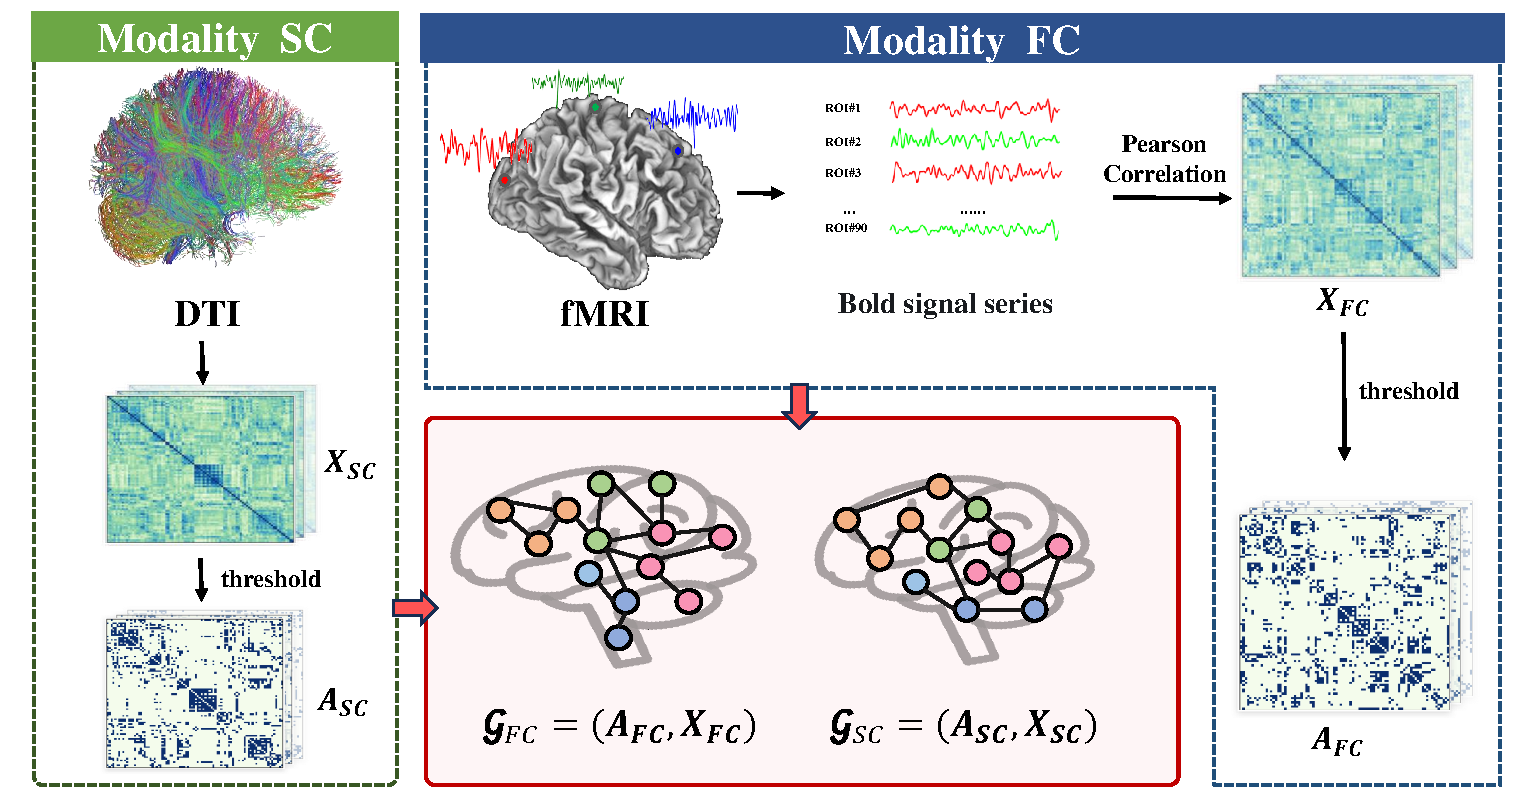
\includegraphics[width=0.96\linewidth]{preprocess.pdf}
    \caption{Multi-modal brain networks construction.}
    \label{pdf_preprocess}
\end{figure}

% \begin{figure*}[!htbp]
%     \centering
%     \begin{subfigure}[b]{0.28\linewidth}
%         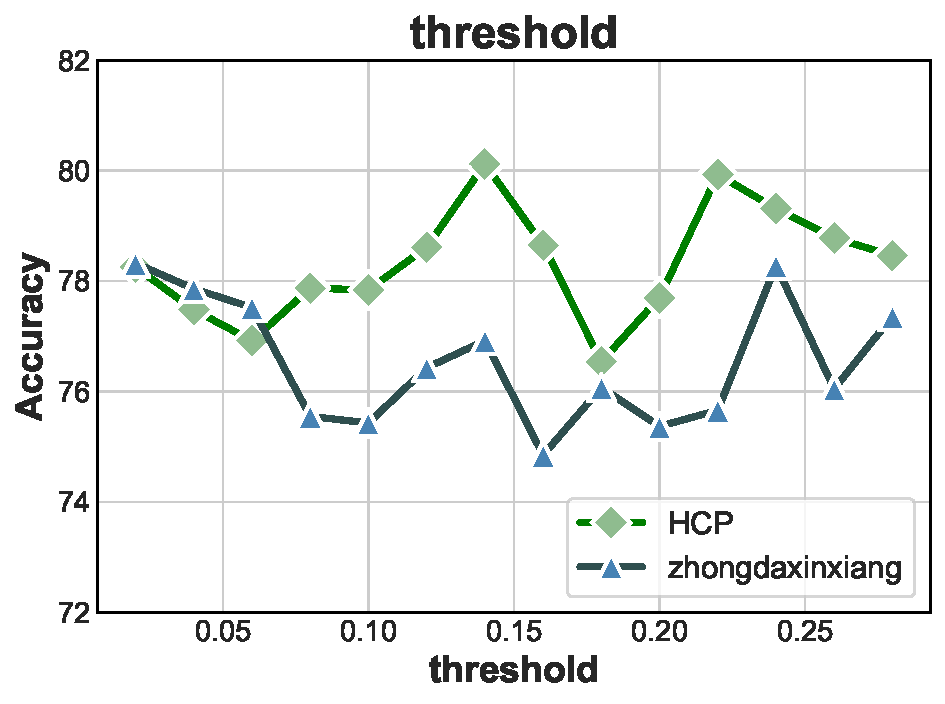
\includegraphics[width=\linewidth]{hyper_threshold.pdf} \caption{} \label{hyper_a}
%     \end{subfigure}
%     \begin{subfigure}[b]{0.33\linewidth}
%         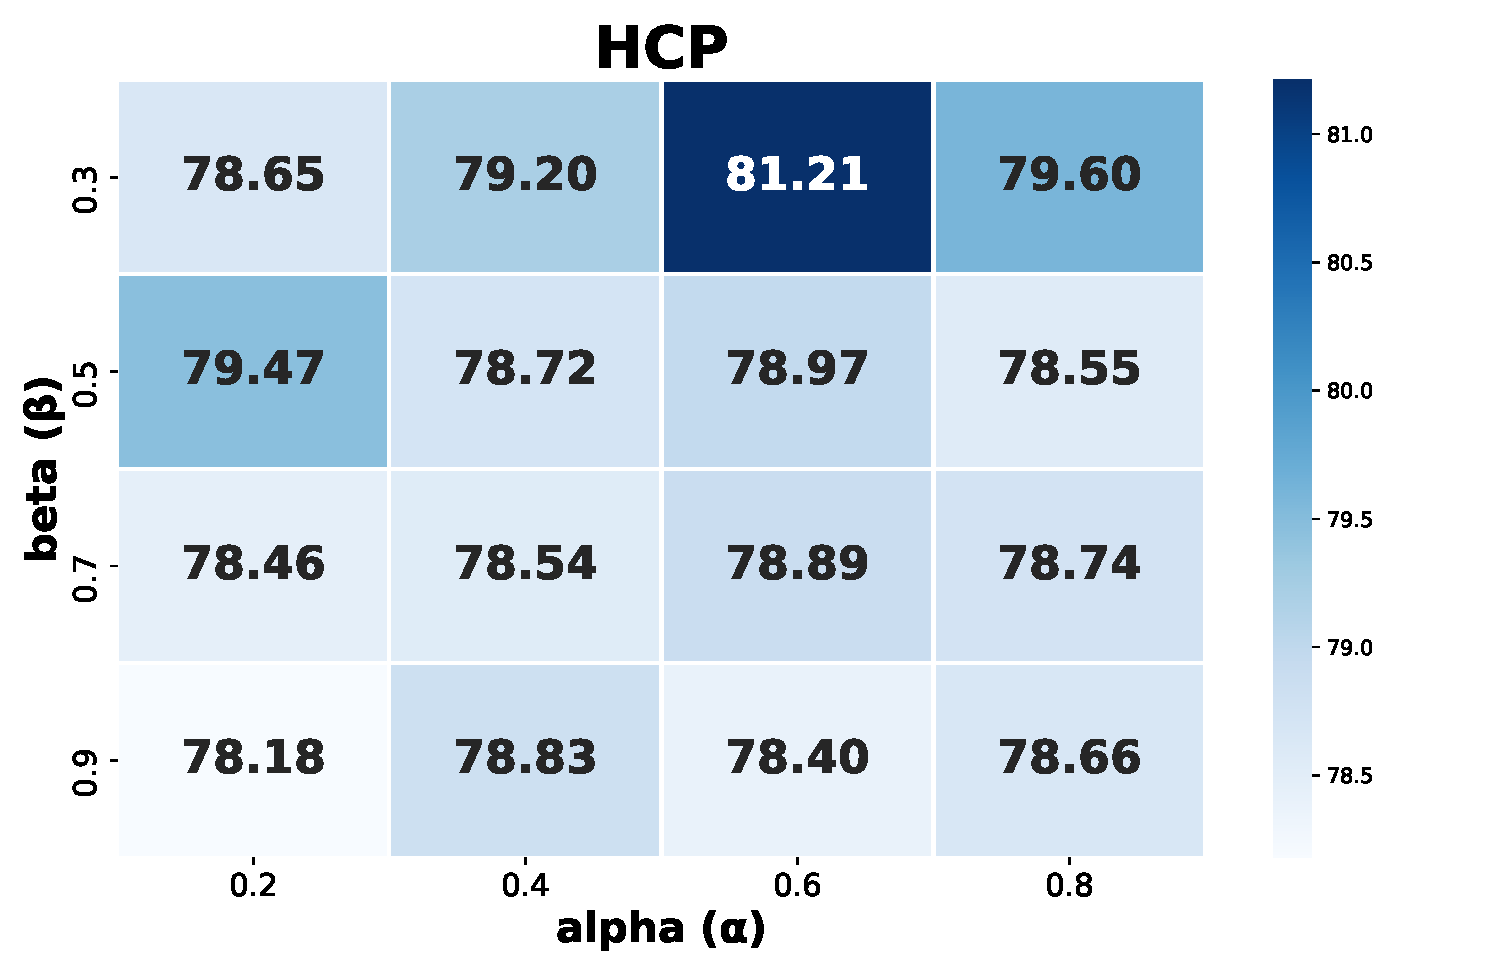
\includegraphics[width=\linewidth]{grid_HCP.pdf} \caption{} \label{hyper_b}
%     \end{subfigure}
%     \begin{subfigure}[b]{0.28\linewidth}

%         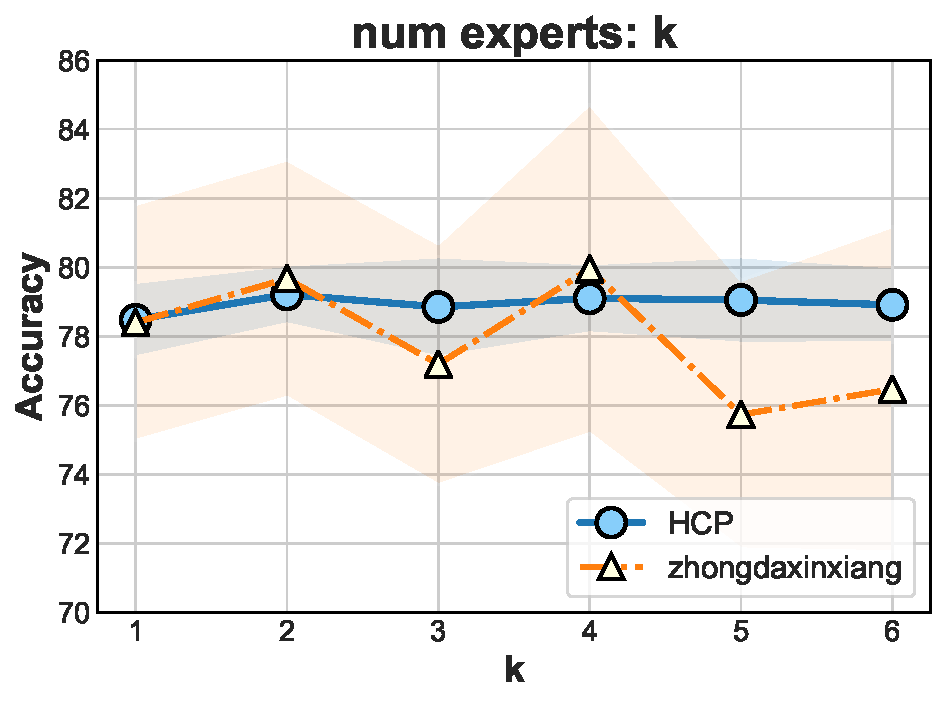
\includegraphics[width=\linewidth]{hyper_k.pdf} \caption{} \label{hyper_c}
%     \end{subfigure}

%     \caption{Experiment results on different hyper-parameters. (a) for threshold, (b) for $\alpha, \beta$ and (c) for expert numbers.}
%     \label{fig_hyper-parameter}
% \end{figure*}

\vspace{0.35em}
\noindent\textbf{Baselines.} 
% For baselines on comparison experiments, we both select uni-modal encoders and multi-modal brain fusion models. 
For uni-modal methods, as we choose \textbf{GCN} as our uni-modal encoders, we record its results in uni-modal scenes. Besides, we select \textbf{BrainNPT} \cite{hu2024brainnpt}, a transformer-based method for brain network analysis. For multi-modal methods, we select (1) 2 methods which concatenate SC/FC features as input: \textbf{SVM}, \textbf{Random Forest}; (2) 1 method concatenates uni-modal embeddings: \textbf{MMGNN} \cite{sebenius2021multimodal}; (3) 2 methods which construct a graph between different modalities for fusion: \textbf{AL-NEGAT} \cite{chen2022adversarial}, \textbf{Cross-GNN} \cite{yang2023mapping} and (4) 2 transformer-based fusion methods: \textbf{RH-BrainFS} \cite{ye2024rh} and \textbf{NeuroPath} \cite{wei2024neuropath}. Code implementations of all baseline methods are taken from their respective original papers. 

\vspace{0.35em}
\noindent\textbf{Experimental settings.} We choose 3-layer GCN with its hidden dimension 128 for uni-modal encoders. For fusion parts, we utilize a two-layer MoE. Top-k value of each MoE block is set as 1. We adopt Adam as optimizer and training epochs is 500 in total with 300 epochs as early stopping. For hyper-parameters settings, $\alpha \in \{0.2, 0.4, 0.6, 0.8\}, \beta \in \{0.3, 0.5, 0.7, 0.9\}$. The number of experts in MoE $k \in [2, 6]$. The learning rate is 0.005 with weight dacay as 0.0001. Our model is implemented in PYG and trained on RTX Titans with 24GB memory. 

We evaluate model's performance on five metrics: accuracy (\textbf{ACC}), sensitivity (\textbf{SEN}), specificity (\textbf{SPE}), f1 score (\textbf{F1}) and ROC-AUC (\textbf{AUC}), where higher value means better performance. We use 10-fold cross validation on 10 random runs and record mean value and standard deviation.

%================== table-ablation=====================%
% \subfile{table-ablation.tex}
\begin{table}[!htbp]
    \centering
    \caption{Ablation studies on sub-stages and sub-modules.}
    \resizebox{\linewidth}{!}{
    \begin{tabular}{c|cccc|cc}
        \toprule
        \multirow{2}{*}{\textbf{Ablation types}} &
        \multicolumn{1}{c|}{\textbf{Stage 1}} & 
        \multicolumn{2}{c|}{\textbf{Stage 2}} & 
        \multicolumn{1}{c|}{\textbf{Stage 3}} &
        \multicolumn{2}{c}{\textbf{Datasets}}
        \\
         & \multicolumn{1}{c|}{\small\textit{KD}}  & \small\textit{pretrain} & \multicolumn{1}{c|}{\small$\mathcal{L}_{contrast}$} & \small$\mathcal{L}_{disen}$ & HCP & zhongdaxinxiang
        \\
        % & $\mathcal{L}_{intra}$ & $\mathcal{L}_{inter}$  & Cora & Pubmed & Computers & CS  \\ 
        
        \midrule
        $S_1.A_1$ & \XSolidBrush & \XSolidBrush & \XSolidBrush & \XSolidBrush & 76.84 $\pm$ \scriptsize{1.92} & 77.28 $\pm$ \scriptsize{4.71}\\
        $S_2.A_1$ & \Checkmark & \XSolidBrush & \XSolidBrush & \XSolidBrush & 78.16 $\pm$ \scriptsize{1.57} & 79.67 $\pm$ \scriptsize{4.42}\\
        $S_2.A_2$ & \Checkmark & \Checkmark & \XSolidBrush & \XSolidBrush & 78.57 $\pm$ \scriptsize{1.06} & 77.00 $\pm$ \scriptsize{2.52}\\
        $S_3.A_1$ & \Checkmark & \Checkmark & \Checkmark & \XSolidBrush & 77.80 $\pm$ \scriptsize{1.22} & 78.68 $\pm$ \scriptsize{4.06}\\
        \midrule
        \textbf{M$^3$D-BFS} & \Checkmark & \Checkmark & \Checkmark & \Checkmark & \textbf{81.21 $\pm$ \scriptsize{0.85}} & \textbf{80.85 $\pm$ \scriptsize{2.44}}\\
        \bottomrule
    \end{tabular}    
    } 
    \label{tab_ablation}
\end{table}

%========================end table======================%

\begin{figure}[H]
    \centering
    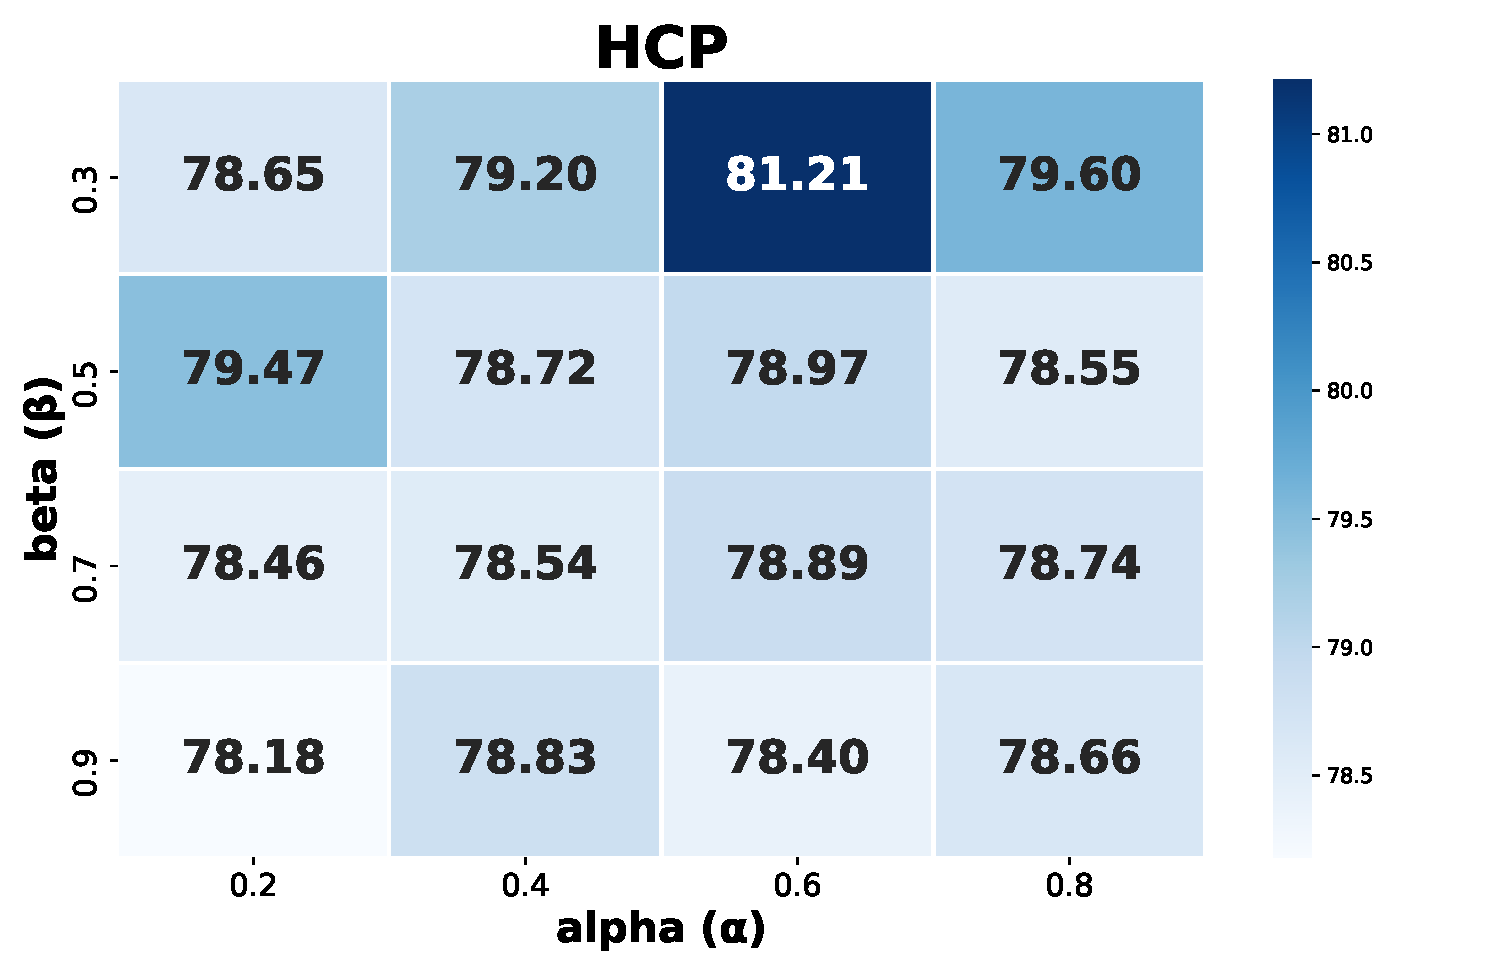
\includegraphics[width=0.47 \linewidth]{grid_HCP.pdf}
    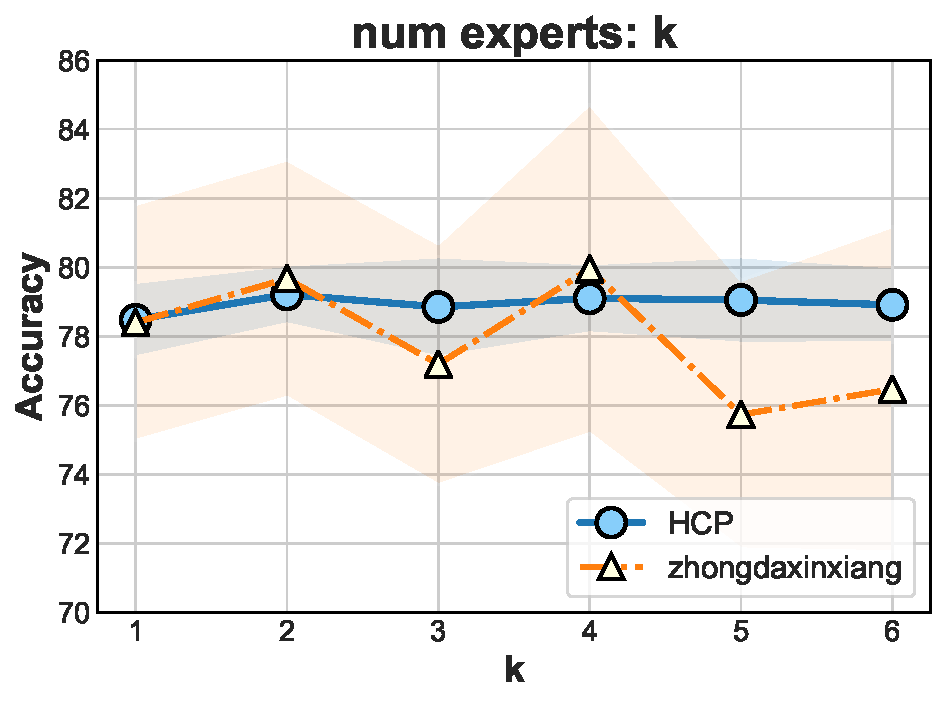
\includegraphics[width=0.47\linewidth]{hyper_k.pdf}
    
    \caption{Sensitivity analysis experiments.}
    \label{fig_hyper}
\end{figure}

\begin{figure}[H]
    \centering
    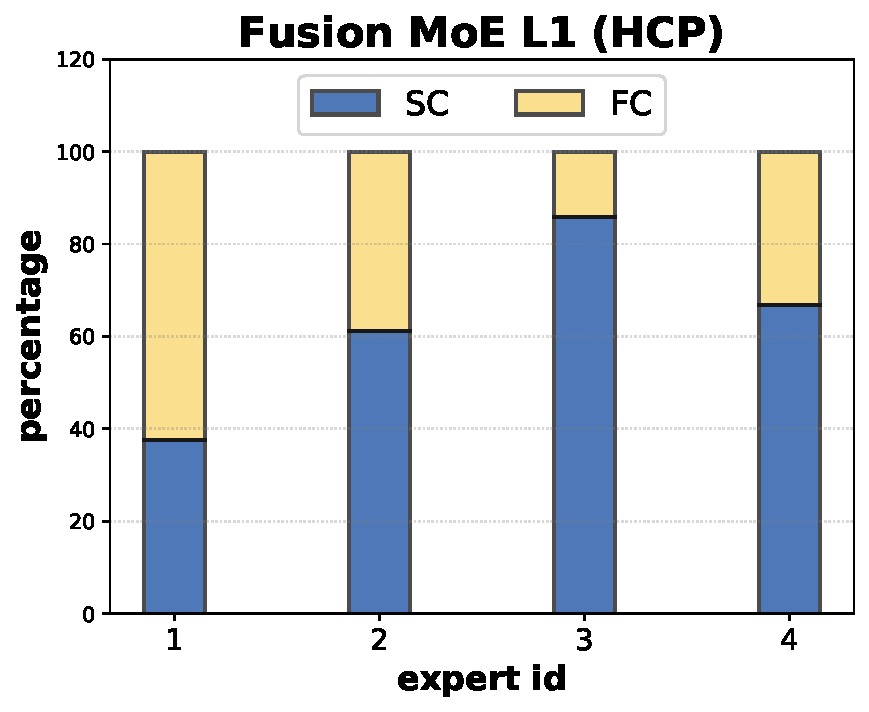
\includegraphics[width=0.43\linewidth]{moe_HCP_1.pdf}
    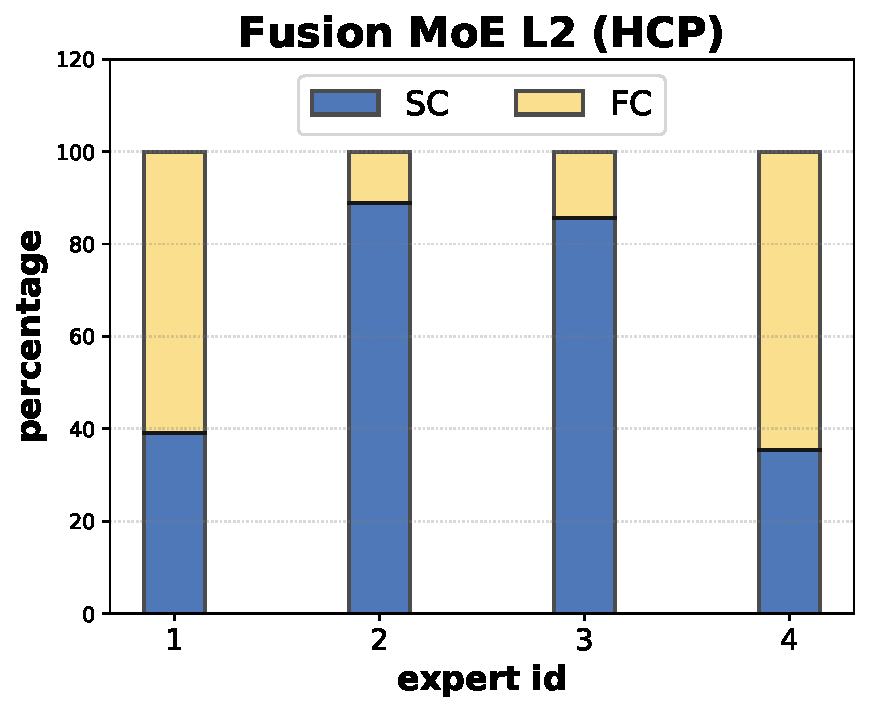
\includegraphics[width=0.43\linewidth]{moe_HCP_2.pdf}
    \\
    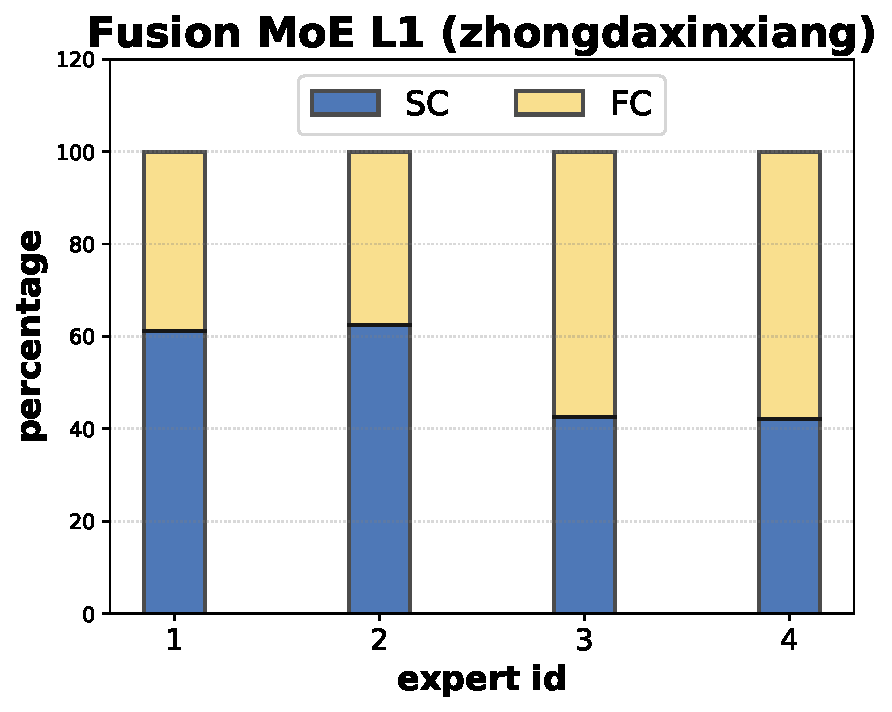
\includegraphics[width=0.43\linewidth]{moe_ZDXX_1.pdf}
    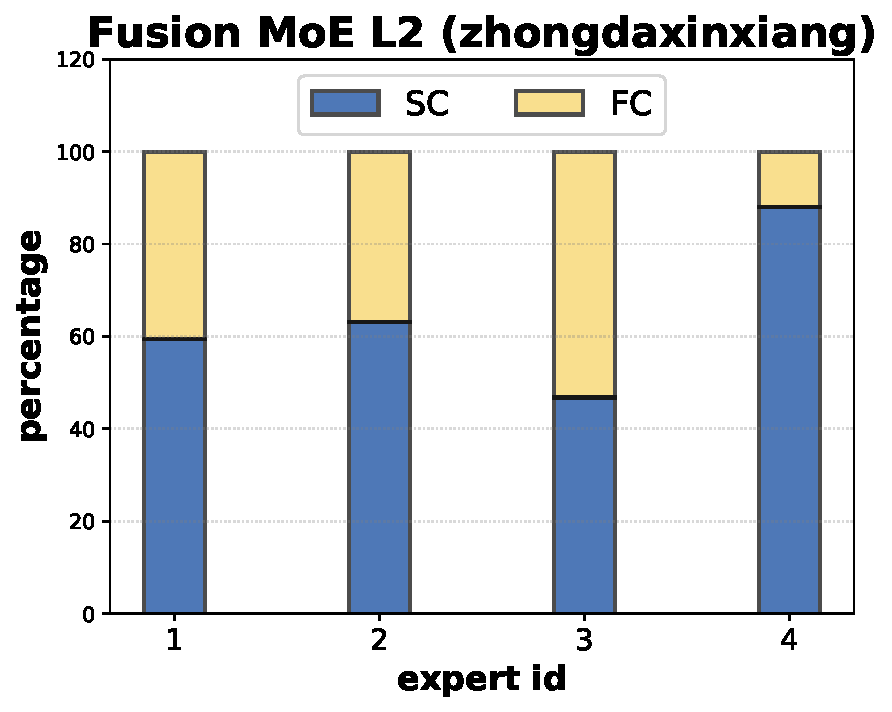
\includegraphics[width=0.43\linewidth]{moe_ZDXX_2.pdf}
    
    \caption{Visualization for uni-modal percentage (SC:FC) in each fusion MoE block.}
    \label{fig_moe_fusion}
\end{figure}

\begin{figure*}[!htbp]
    \centering
    \begin{subfigure}[b]{0.22\linewidth}
        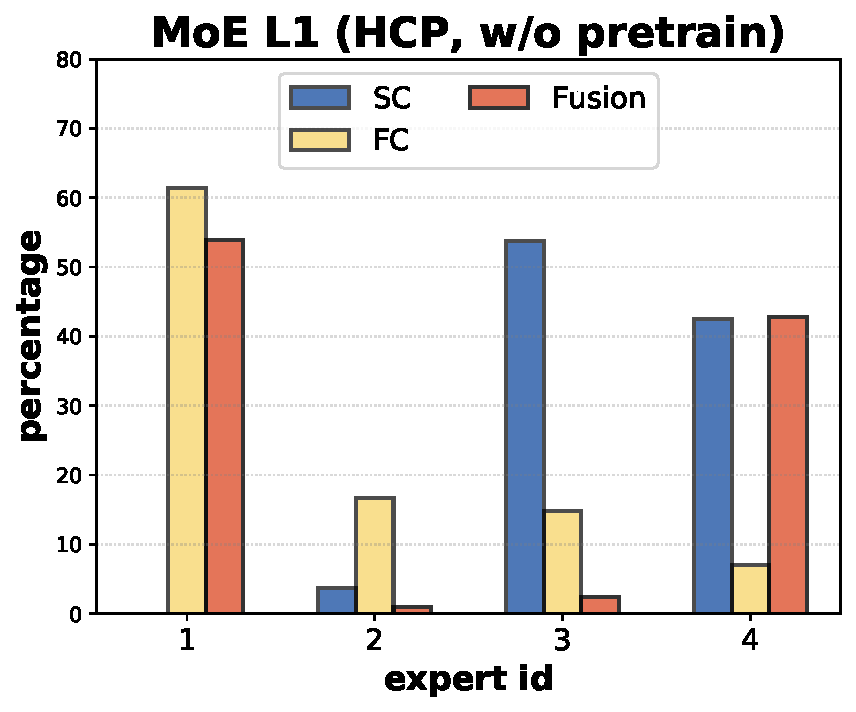
\includegraphics[width=\linewidth]{moe_HCP_1_abl.pdf} \caption{} \label{a}
    \end{subfigure}
    \begin{subfigure}[b]{0.22\linewidth}
        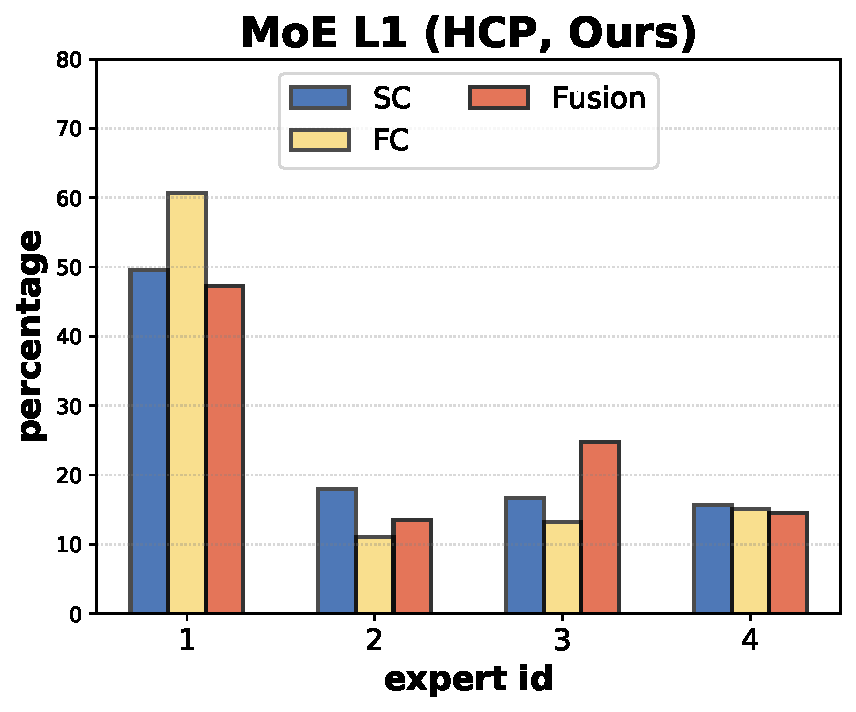
\includegraphics[width=\linewidth]{moe_HCP_1_ours.pdf} \caption{} \label{b}
    \end{subfigure}
    \begin{subfigure}[b]{0.22\linewidth}
        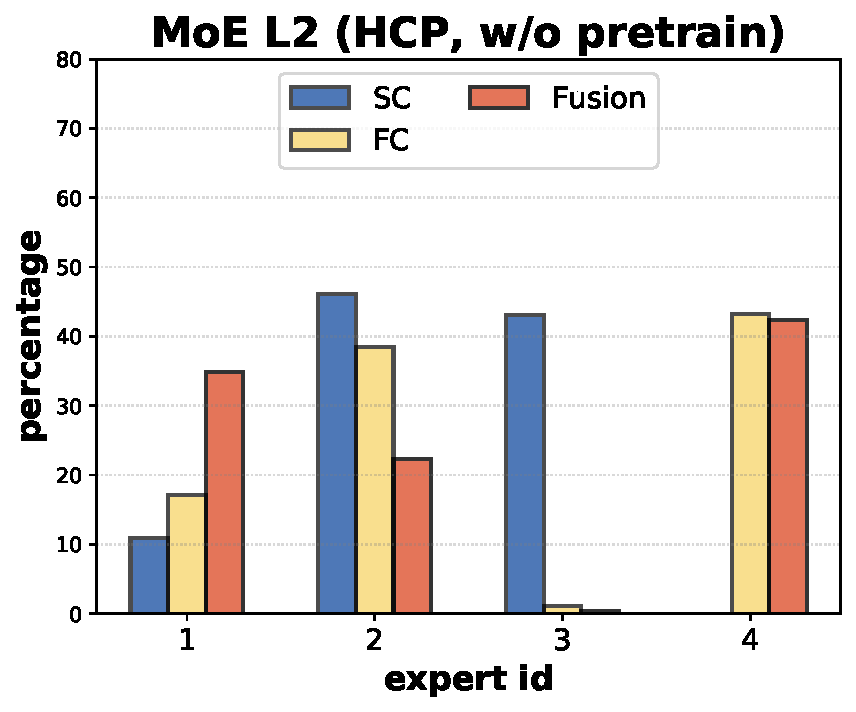
\includegraphics[width=\linewidth]{moe_HCP_2_abl.pdf} \caption{} \label{c}
    \end{subfigure}
    \begin{subfigure}[b]{0.22\linewidth}
        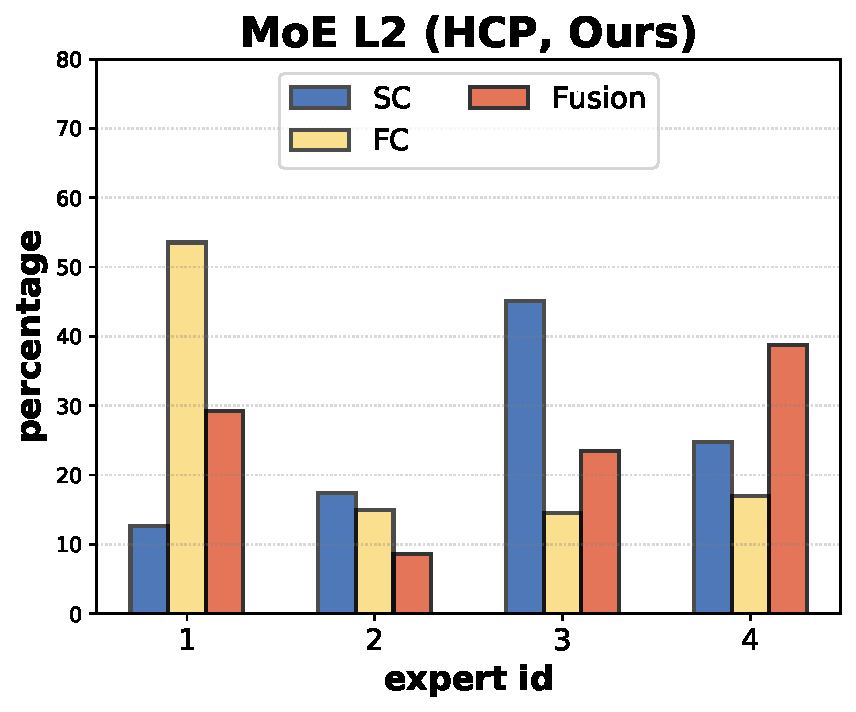
\includegraphics[width=\linewidth]{moe_HCP_2_ours.pdf} \caption{} \label{d}
    \end{subfigure}


    \begin{subfigure}[b]{0.22\linewidth}
        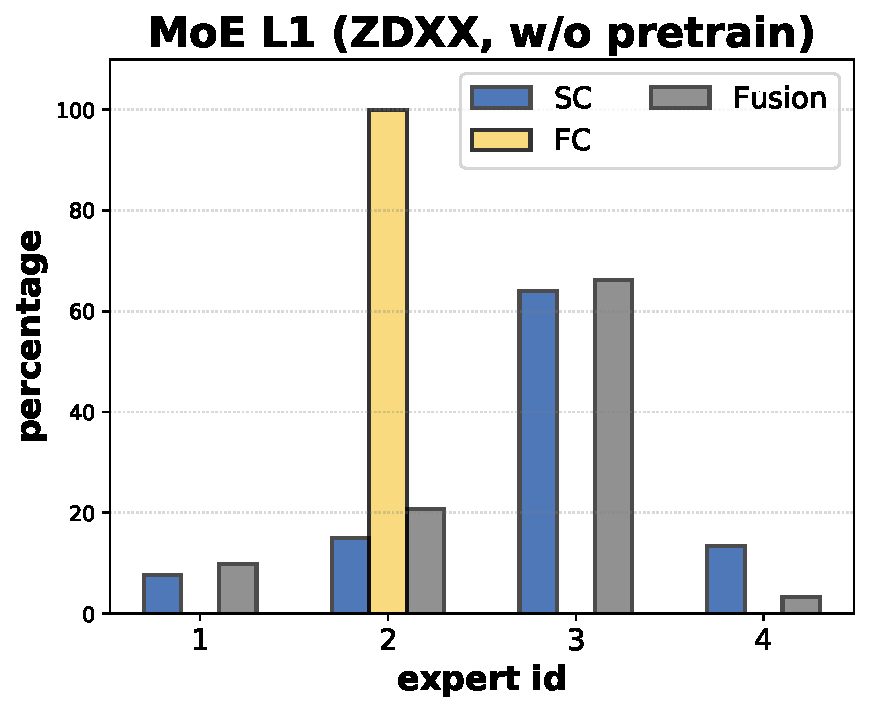
\includegraphics[width=\linewidth]{moe_ZDXX_1_abl.pdf} \caption{} \label{e}
    \end{subfigure}
    \begin{subfigure}[b]{0.22\linewidth}
        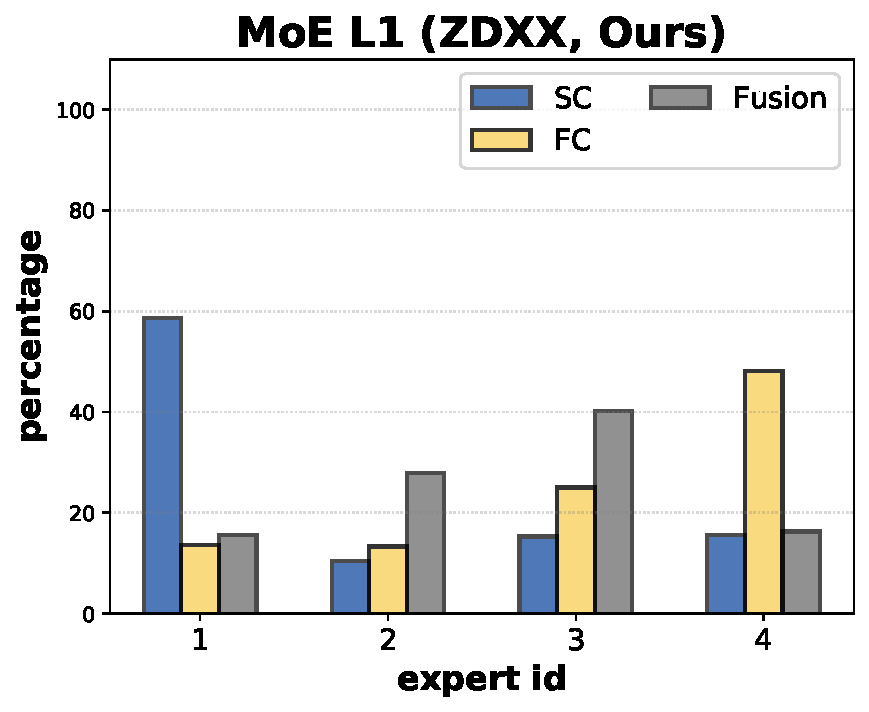
\includegraphics[width=\linewidth]{moe_ZDXX_1_ours.pdf} \caption{} \label{f}
    \end{subfigure}
    \begin{subfigure}[b]{0.22\linewidth}
        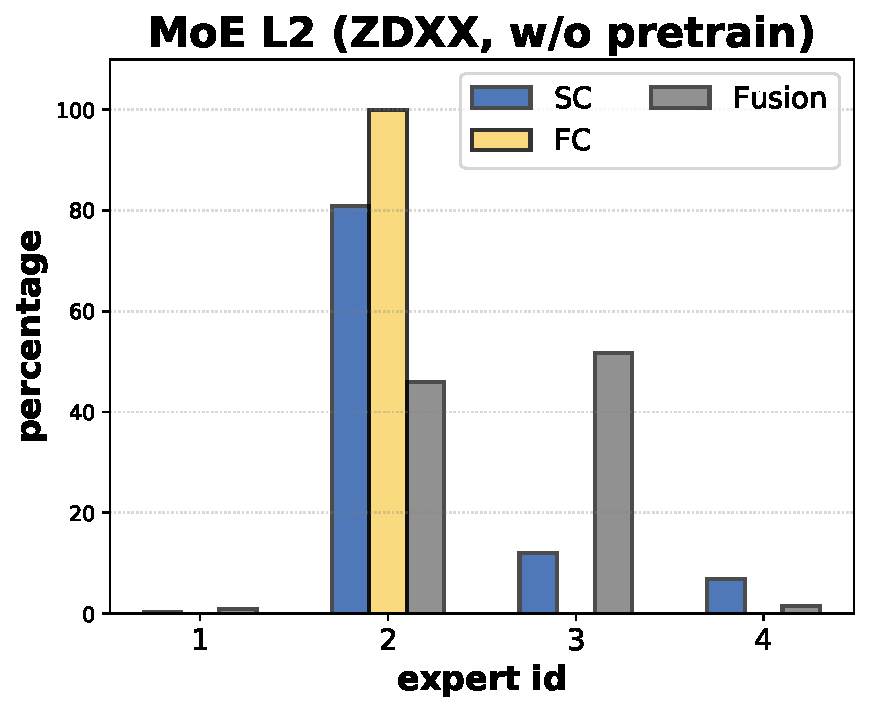
\includegraphics[width=\linewidth]{moe_ZDXX_2_abl.pdf} \caption{} \label{g}
    \end{subfigure}
    \begin{subfigure}[b]{0.22\linewidth}
        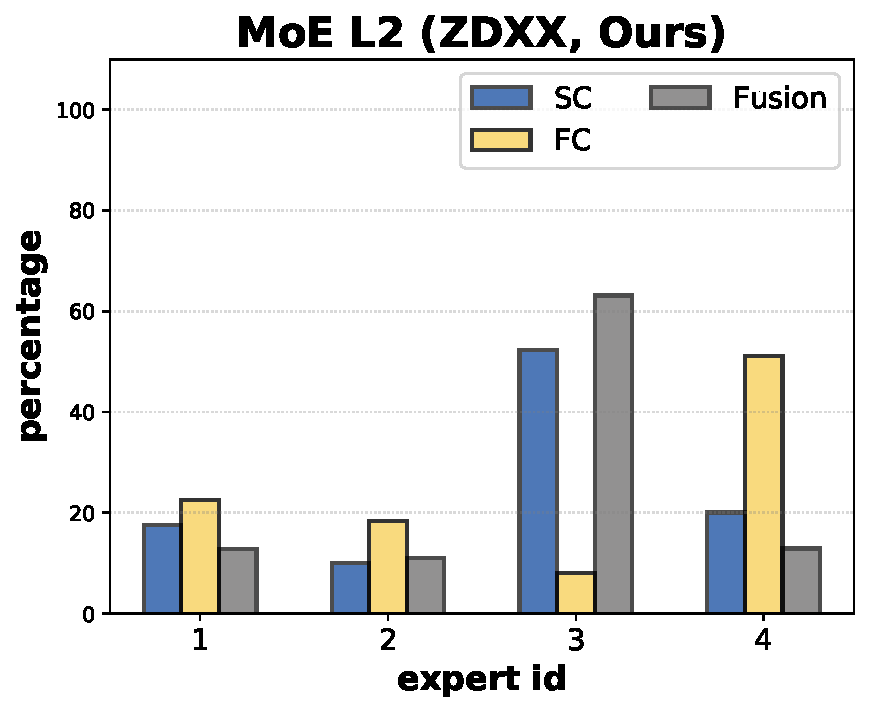
\includegraphics[width=\linewidth]{moe_ZDXX_2_ours.pdf} \caption{} \label{h}
    \end{subfigure}

    \caption{Visualization for percentage of experts in different MoEs. Here each MoE consists of 4 experts.}
    \label{fig_moe_all}
\end{figure*}

\subsection{Comparison experiments}
The results of different methods for two datasets are shown in Tab. \ref{table_comp_HCP}. Compared to uni-modal GCNs, \model greatly outperforms uni-modal encoders.
% which is a good answer to \textbf{Q1}. 
Moreover, compared to other multi-modal brain fusion methods, \model also performs the best (2.28\% \textbf{ACC} improvement on HCP and 2.73\% \textbf{ACC} improvement on ZDXX). 
% Compared with latest transformer-based methods, our model which uses only MLPs for fusion, can reach higher performance with less GPU requirements. 
% The comparison results in Tab. \ref{table_comp_HCP} greatly answer \textbf{Q2}.


\subsection{Ablation studies and sensitivity analyses}
We conduct ablation studies to illustrate effectiveness of different sub-modules in M$^3$D-BFS. 
We validate its effectiveness via stage-by-stage ablation. As is shown in Tab. \ref{tab_ablation}, $S_i.A_j$ means ablation for stage $i$ and $j\mbox{-}th$ sub-module in stage $i$. The results in Tab. \ref{tab_ablation} show that each sub-module works in our M$^3$D-BFS. The distillation from uni-modal encoders ensure the models' representations for uni-modal during fusion ($S_1.A_1$). The ``pretrain-finetune'' method not only improves accuracy, but also lowers deviation ($S_2.A_1, S_2.A_2$). Finally $\mathcal{L}_{disen}$ leads to better performance ($S_3.A_1$). 
% The ablation study result is a good answer to \textbf{Q3}.

% To answer \textbf{Q4}, 
% We conduct extensive experiments on different hyper-parameters. 
% Our experiments include: (1) \textbf{threshold} for graph construction in the preprocess part, (2) \textbf{coefficients} for loss function \textbf{$(\alpha, \beta)$} and (3) number of experts \textbf{k} for MoE block. 
% For threshold, we set the value range of threshold between [0.02, 0.30], with 0.02 as step size. The results are plot in Fig. \ref{fig_hyper-parameter} (a). In the experiment, we set threshold value as 0.12 for default, while the threshold value for best performance varies for different datasets.
We also conduct extensive experiments on different hyper-parameters. 
For loss function coefficients, here we consider $\beta$ in stage 2 and $\alpha$ in stage 3 and plot the heatmap for them, which is depicted in Fig. \ref{fig_hyper}. For HCP, the accuracy reaches its peak when the values are $(\alpha, \beta) = (0.6, 0.3)$.
Finally we conduct experiments on different expert numbers in the MoE block. The value of number k is from 1 to 6, and as is shown in Fig. \ref{fig_hyper}, for HCP, the change of accuracy is subtler than ZDXX dataset.

% \begin{figure}[H]
%     \centering
%     % 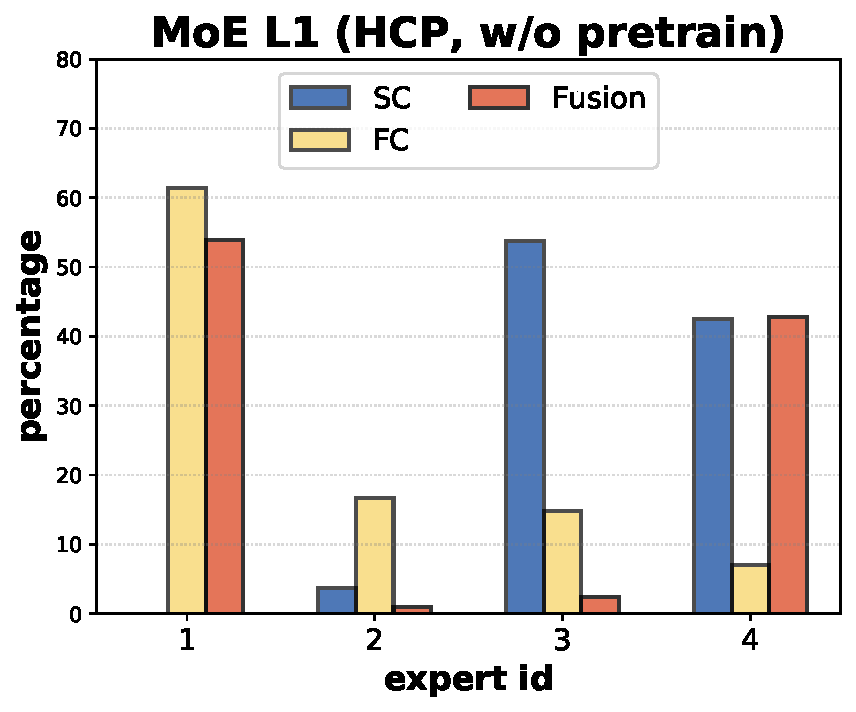
\includegraphics[width=0.44\linewidth]{moe_HCP_1_abl.pdf}
%     % 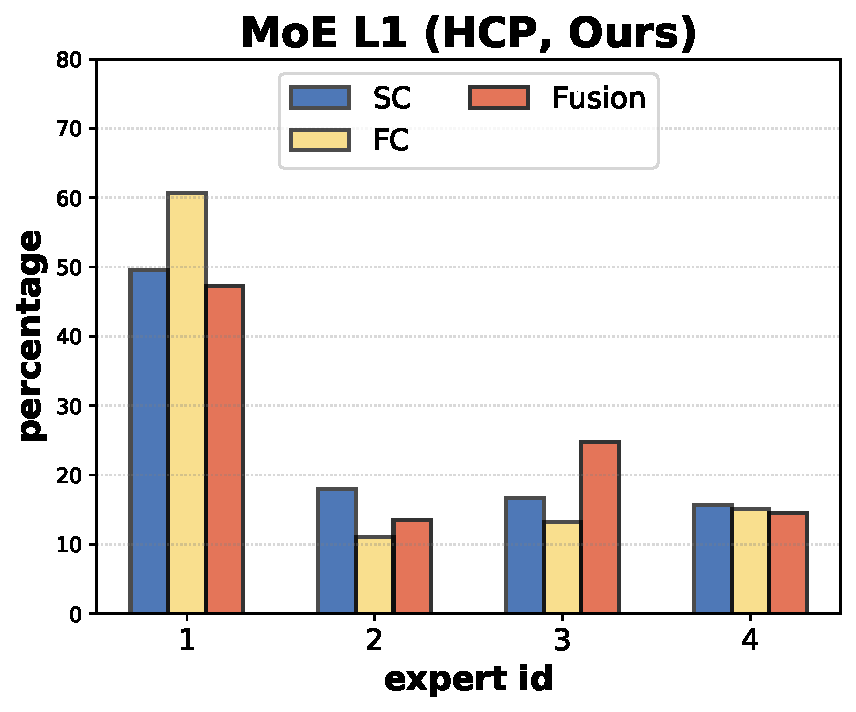
\includegraphics[width=0.44\linewidth]{moe_HCP_1_ours.pdf}
%     % \\
%     % 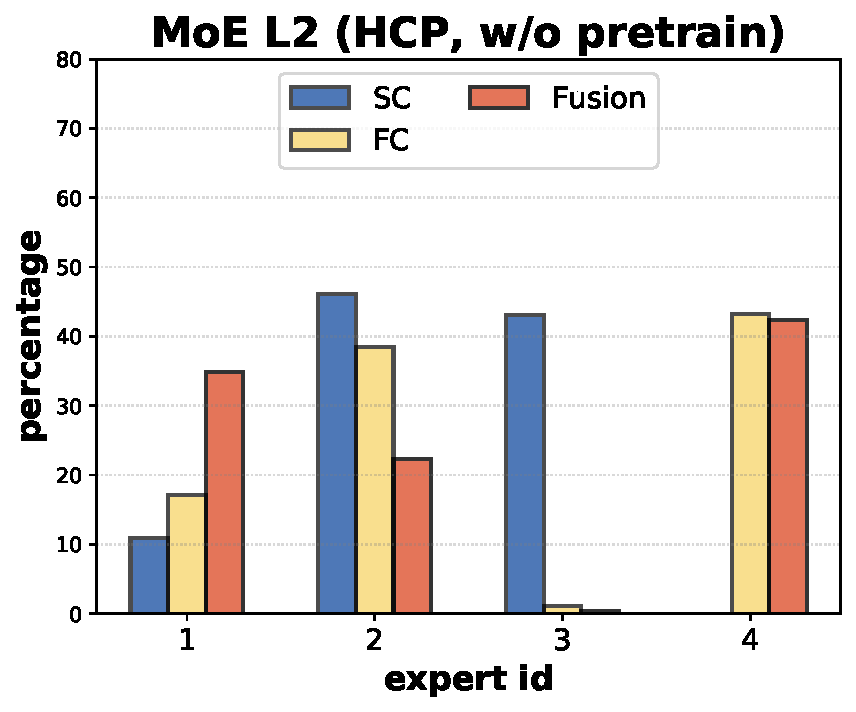
\includegraphics[width=0.44\linewidth]{moe_HCP_2_abl.pdf}
%     % 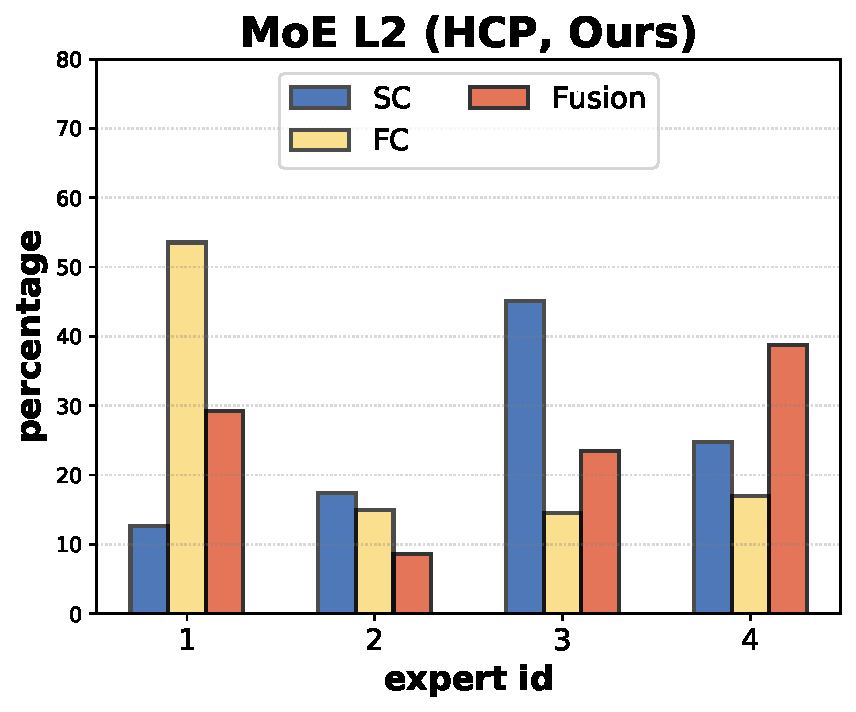
\includegraphics[width=0.44\linewidth]{moe_HCP_2_ours.pdf}
%     % \\
%     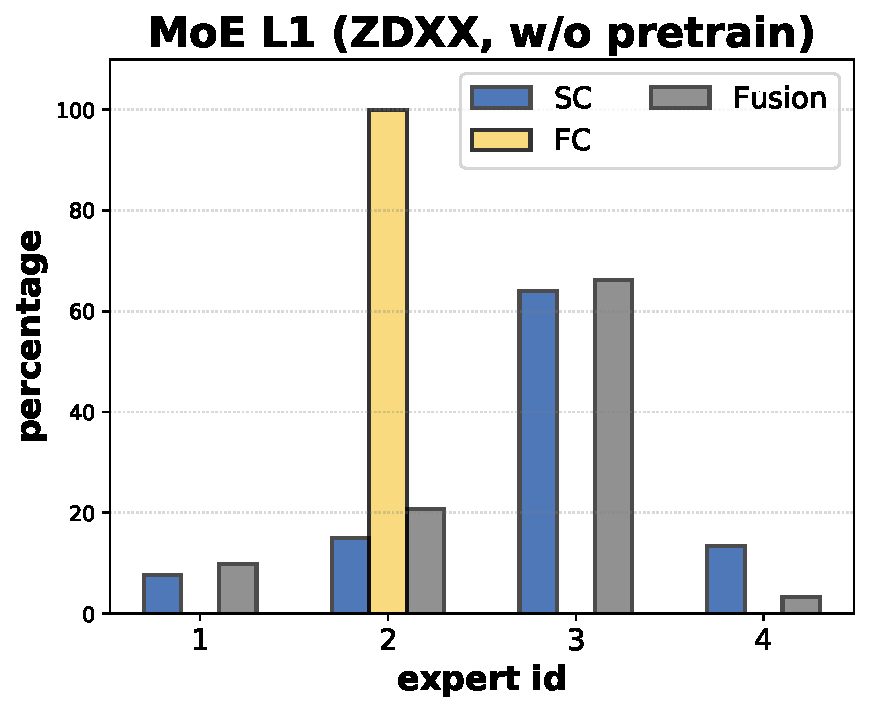
\includegraphics[width=0.44\linewidth]{moe_ZDXX_1_abl.pdf}
%     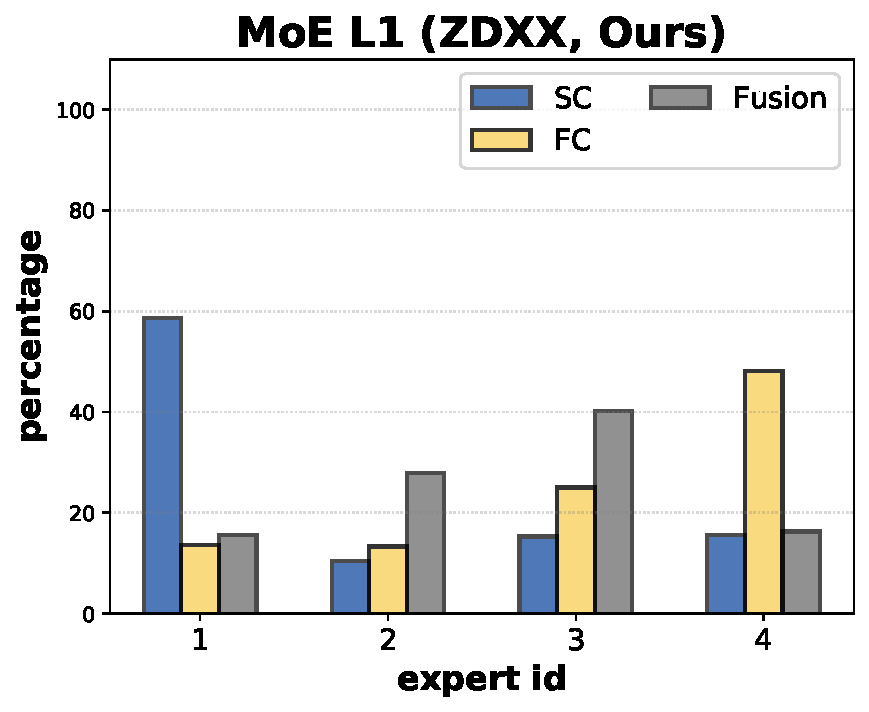
\includegraphics[width=0.44\linewidth]{moe_ZDXX_1_ours.pdf}
%     \\
%     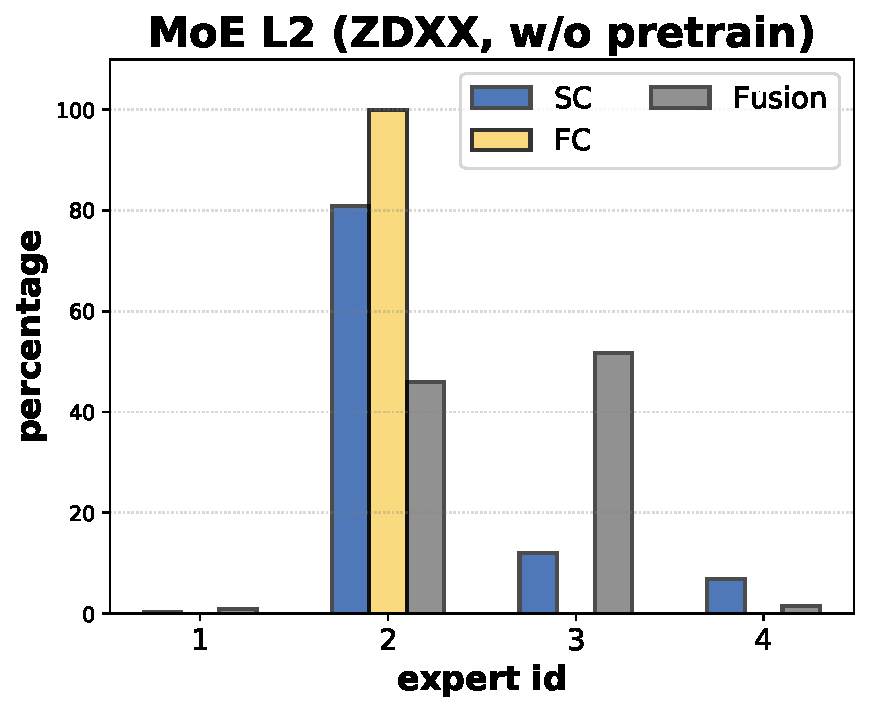
\includegraphics[width=0.44\linewidth]{moe_ZDXX_2_abl.pdf}
%     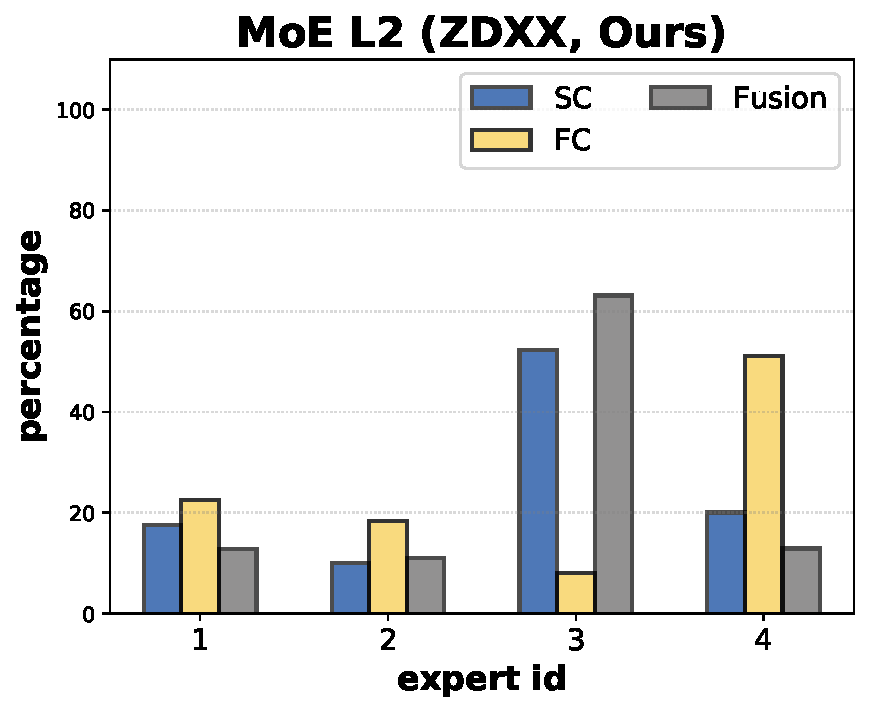
\includegraphics[width=0.44\linewidth]{moe_ZDXX_2_ours.pdf}
%     \caption{Visualization for percentage of experts in different MoEs. (ZDXX)}
%     \label{fig_moe_all_ZDXX}
% \end{figure}


\subsection{Visualization for experts}
% Finally, we plot distributions of the routing network from MoE blocks for visualization. Here we select cases where number if experts is 4. 
Firstly we plot percentage of different modalities in each fusion MoE block. As is shown in Fig. \ref{fig_moe_fusion}, every fusion expert avoid collapse (SC/FC 100\% or 0\%) phenomenon, showing that \model \textbf{gets effective training in dynamic fusion}. Then we plot the distribution of all experts in one MoE block to check if expert collapse occurs in our model. We also plot distributions for models without pretraining (left side) in stage 2 as comparison, which is shown in Fig. \ref{fig_moe_all}. For MoE in both layers, model without pretraining may face collapse among experts. While for M$^3$D-BFS (right side), the issue is effectively mitigated, \textbf{with more even distributions for different experts}. 


\section{Conclusion}
 In this work, we propose a multi-stage MoE-based multi-modal brain network fusion method (M$^3$D-BFS) for sample-adaptive dynamic fusion in neuroscience. To the best of our knowledge, this is the first paper discussing dynamic fusion in multi-modal brain fusion. Extensive experiments on different real-world datasets validate the effectiveness of our method. In our future work, we aim to consider more complex cases where different data may have inherent bias in its distribution to achieve better results in different downstream tasks under multi-modal brain network scenarios.


% \section*{Ethical Statement}
% \textbf{Possible ethical issues for datasets.} For HCP, as a public dataset and have been widely used in previous researches. For zhongdaxinxiang, it is held in collaboration with our partner and is not yet publicly available, but the data is collected with the consent of the subjects who are clearly informed of the purpose of the sample collection, and all identifying information about the sample is hidden in the hospital dataset. Therefore, there are no ethical issues for our datasets.

\section*{Acknowledgement}
This work is supported by National Natural Science Foundation of China (Grant No.62471133). 
This work is also supported by the Big Data Computing Center of Southeast University.

{
    \small
    \bibliographystyle{ieeenat_fullname}
    \bibliography{references}
}

% WARNING: do not forget to delete the supplementary pages from your submission 
% \input{sec/X_suppl}

\end{document}
